%%
%% This is file `sample-acmsmall.tex',
%% generated with the docstrip utility.
%%
%% The original source files were:
%%
%% samples.dtx  (with options: `all,journal,bibtex,acmsmall')
%%
%% IMPORTANT NOTICE:
%%
%% For the copyright see the source file.
%%
%% Any modified versions of this file must be renamed
%% with new filenames distinct from sample-acmsmall.tex.
%%
%% For distribution of the original source see the terms
%% for copying and modification in the file samples.dtx.
%%
%% This generated file may be distributed as long as the
%% original source files, as listed above, are part of the
%% same distribution. (The sources need not necessarily be
%% in the same archive or directory.)
%%
%%
%% Commands for TeXCount
%TC:macro \cite [option:text,text]
%TC:macro \citep [option:text,text]
%TC:macro \citet [option:text,text]
%TC:envir table 0 1
%TC:envir table* 0 1
%TC:envir tabular [ignore] word
%TC:envir displaymath 0 word
%TC:envir math 0 word
%TC:envir comment 0 0
%%
%% The first command in your LaTeX source must be the \documentclass
%% command.
%%
%% For submission and review of your manuscript please change the
%% command to \documentclass[manuscript, screen, review]{acmart}.
%%
%% When submitting camera ready or to TAPS, please change the command
%% to \documentclass[sigconf]{acmart} or whichever template is required
%% for your publication.
%%
%%
% \documentclass[acmsmall]{acmart}
% \documentclass[manuscript]{acmart}
\documentclass[acmsmall, screen]{acmart}

\usepackage{amsmath, amsfonts}
\usepackage{algorithm}
% \usepackage{algorithmic}
\usepackage{array}
\usepackage[caption=false, font=normalsize, labelfont=sf, textfont=sf]{subfig}
\usepackage{textcomp}
\usepackage{stfloats}
\usepackage{url}
\usepackage{verbatim}
\usepackage{graphicx}
\usepackage{hyperref}
\usepackage{textcomp}
\usepackage{xcolor}
\usepackage{tabularx}
\usepackage{listings}
\usepackage{multirow}
\usepackage{enumitem}
% \usepackage{hyperref}
\usepackage{pifont}
\usepackage[breakable]{tcolorbox}
\usepackage{adjustbox}
\usepackage{booktabs}
\usepackage[flushleft]{threeparttable}
\usepackage[noend]{algpseudocode}

\usepackage{xurl}
\def\UrlBreaks{%
	\do\/%
	\do\a\do\b\do\c\do\d\do\e\do\f\do\g\do\h\do\i\do\j\do\k\do\l%
	\do\m\do\n\do\o\do\p\do\q\do\r\do\s\do\t\do\u\do\v\do\w\do\x\do\y\do\z%
	\do\A\do\B\do\C\do\D\do\E\do\F\do\G\do\H\do\I\do\J\do\K\do\L%
	\do\M\do\N\do\O\do\P\do\Q\do\R\do\S\do\T\do\U\do\V\do\W\do\X\do\Y\do\Z%
	\do0\do1\do2\do3\do4\do5\do6\do7\do8\do9\do=\do/\do.\do:%
	\do\*\do\-\do\~\do\'\do\"\do\-}
\urlstyle{same}

% Define custom colors
\definecolor{mylinkcolor}{RGB}{0, 0, 0} % Black color for links
\definecolor{mycitecolor}{RGB}{128, 0, 128} % Purple color for citation links
\definecolor{mycitebg}{RGB}{173, 216, 230} % Light blue color for citation background

% Set up hyperref with custom colors
\hypersetup{
	colorlinks=true, % false: boxed links; true: colored links
	linkcolor=mylinkcolor, % color of internal links (change box color with linkbordercolor)
	citecolor=mycitecolor, % color of citation links
	urlcolor=mylinkcolor, % color of external links
	linkbordercolor=mycitebg % background color for citation links
}

\definecolor{verylightgray}{rgb}{.97,.97,.97}
\lstdefinelanguage{Solidity}{ keywords=[1]{ anonymous, assembly, assert, balance, break, call, callcode, case, catch, class, constant, continue, constructor, contract, debugger, default, delegatecall, delete, do, else, emit, event, experimental, export, external, false, finally, for, function, gas, if, implements, import, in, indexed, instanceof, interface, internal, is, length, library, log0, log1, log2, log3, log4, memory, modifier, new, payable, pragma, private, protected, public, pure, push, require, return, returns, revert, selfdestruct, send, solidity, storage, struct, suicide, super, switch, then, this, throw, transfer, true, try, typeof, using, value, view, while, with, addmod, ecrecover, keccak256, mulmod, ripemd160, sha256, sha3}, % generic keywords including crypto operations
	keywordstyle=[1]
	\color{blue}
	\bfseries, keywords=[2]{ address, bool, byte, bytes, bytes1, bytes2, bytes3, bytes4, bytes5, bytes6, bytes7, bytes8, bytes9, bytes10, bytes11, bytes12, bytes13, bytes14, bytes15, bytes16, bytes17, bytes18, bytes19, bytes20, bytes21, bytes22, bytes23, bytes24, bytes25, bytes26, bytes27, bytes28, bytes29, bytes30, bytes31, bytes32, enum, int, int8, int16, int24, int32, int40, int48, int56, int64, int72, int80, int88, int96, int104, int112, int120, int128, int136, int144, int152, int160, int168, int176, int184, int192, int200, int208, int216, int224, int232, int240, int248, int256, mapping, string, uint, uint8, uint16, uint24, uint32, uint40, uint48, uint56, uint64, uint72, uint80, uint88, uint96, uint104, uint112, uint120, uint128, uint136, uint144, uint152, uint160, uint168, uint176, uint184, uint192, uint200, uint208, uint216, uint224, uint232, uint240, uint248, uint256, var, void, ether, finney, szabo, wei, days, hours, minutes, seconds, weeks, years}, % types; money and time units
	keywordstyle=[2]
	\color{teal}
	\bfseries, keywords=[3]{ block, blockhash, coinbase, difficulty, gaslimit, number, timestamp, msg, gas, sender, sig, value, now, tx, gasprice, origin}, % environment variables
	keywordstyle=[3]
	\color{violet}
	\bfseries, keywords=[4]{mload,create,create2,add}, keywordstyle=[4]
	\color{red}
	\bfseries, identifierstyle=
	\color{black}
	, sensitive=true, comment=[l]{//}, morecomment=[s]{/*}{*/}, commentstyle=
	\color{gray}
	\ttfamily, stringstyle=
	\color{red}
	\ttfamily, morestring=[b]', morestring=[b]", }

% 定义代码块样式
\lstdefinestyle{codestyle}{ language=Solidity, % 选择代码块的语言
	basicstyle=\ttfamily\scriptsize, % 设置基本样式,如字体、大小等
	keywordstyle=
	\color{blue}
	, % 设置关键字的样式
	commentstyle=
	\color{green!60!black}
	, % 设置注释的样式
	stringstyle=
	\color{red}
	, % 设置字符串的样式
	breaklines=true, % 允许代码块自动换行
	numbers=left, % 在左侧显示行号
	numberstyle=\tiny
	\color{black}
	, % 设置行号的样式
	stepnumber=1, % 设置行号递增的步长
	frame=single, % 设置代码块的边框
	xleftmargin=15pt, % 设置行号左侧的距离
% backgroundcolor=\color{gray!5}, % 设置代码块的背景颜色
	captionpos=b, % 设置标题位置为底部
}
\lstset{style=codestyle}

\newtcolorbox{answerbox}{ colback=gray!12, % 背景颜色
	colframe=white, % 边框颜色
	arc=4pt, % 圆角半径
	boxrule=0pt, % 边框宽度
	left=6pt, % 左边距
	right=6pt, % 右边距
	boxsep=0pt, % 文本框和内容之间的间距
	breakable, }

% Define custom colors
\definecolor{mylinkcolor}{RGB}{0, 0, 0} % Black color for links
\definecolor{mycitecolor}{RGB}{128, 0, 128} % Purple color for citation links
\definecolor{mycitebg}{RGB}{173, 216, 230} % Light blue color for citation background

%%
%% \BibTeX command to typeset BibTeX logo in the docs
\AtBeginDocument{%
	\providecommand{\BibTeX}{{%
		Bib\TeX}}}

%% Rights management information.  This information is sent to you
%% when you complete the rights form.  These commands have SAMPLE
%% values in them; it is your responsibility as an author to replace
%% the commands and values with those provided to you when you
%% complete the rights form.
\setcopyright{acmlicensed}
\copyrightyear{2025}
\acmYear{2025}
\acmDOI{XXXXXXX.XXXXXXX}

%%
%% These commands are for a JOURNAL article.
% \acmJournal{JACM}
% \acmVolume{37}
% \acmNumber{4}
% \acmArticle{111}
% \acmMonth{8}

%%
%% Submission ID.
%% Use this when submitting an article to a sponsored event. You'll
%% receive a unique submission ID from the organizers
%% of the event, and this ID should be used as the parameter to this command.
%%\acmSubmissionID{123-A56-BU3}

%%
%% For managing citations, it is recommended to use bibliography
%% files in BibTeX format.
%%
%% You can then either use BibTeX with the ACM-Reference-Format style,
%% or BibLaTeX with the acmnumeric or acmauthoryear sytles, that include
%% support for advanced citation of software artefact from the
%% biblatex-software package, also separately available on CTAN.
%%
%% Look at the sample-*-biblatex.tex files for templates showcasing
%% the biblatex styles.
%%

%%
%% The majority of ACM publications use numbered citations and
%% references.  The command \citestyle{authoryear} switches to the
%% "author year" style.
%%
%% If you are preparing content for an event
%% sponsored by ACM SIGGRAPH, you must use the "author year" style of
%% citations and references.
%% Uncommenting
%% the next command will enable that style.
%%\citestyle{acmauthoryear}

%%
%% end of the preamble, start of the body of the document source.
\begin{document}
	%%
	%% The "title" command has an optional parameter,
	%% allowing the author to define a "short title" to be used in page headers.
	\title[Empirical Analysis of Smart Contract Factories on EVM-Compatible Chains]{Empirical
	Analysis of Smart Contract Factories on EVM-Compatible Chains}

	%%
	%% The "author" command and its associated commands are used to define
	%% the authors and their affiliations.
	%% Of note is the shared affiliation of the first two authors, and the
	%% "authornote" and "authornotemark" commands
	%% used to denote shared contribution to the research.
	\author{Ziyue Wang}
	\email{ziyue0530@gmail.com} \orcid{0009-0000-6621-4712}

	\author{ZongWen Shen}
	\email{szw@smail.nju.edu.cn} \orcid{0009-0005-2492-2530}

	\author{Lei Chen}
	\email{willisgarey89@gmail.com} \orcid{0009-0000-9079-3427} \affiliation{%
		\institution{National Key Laboratory for Novel Software Technology, Nanjing University} \city{Nanjing} \state{Jangsu} \country{China} }

	\author{Wei Song}
	\email{wsong@njust.edu.cn} \orcid{0000-0002-4324-3382} \affiliation{%
		\institution{Nanjing University of Science and Technology} \city{Nanjing} \state{Jangsu} \country{China} }

	\author{Jidong Ge}
	\email{gjd@nju.edu.cn} \orcid{0000-0003-1773-0942} \authornote{Corresponding Authors.}
	\affiliation{%
		\institution{National Key Laboratory for Novel Software Technology, Nanjing University} \city{Nanjing} \state{Jangsu} \country{China} }

	\author{LiGuo Huang}
	\email{lghuang@lyle.smu.edu} \orcid{0000-0001-7790-0195} \affiliation{%
		\institution{Department of Computer Science, Southern Methodist University} \city{Dallas} \state{Texas} \country{USA}}

	\author{Bin Luo}
	\email{luobin@nju.edu.cn} \orcid{0000-0002-9036-0063} \affiliation{%
		\institution{National Key Laboratory for Novel Software Technology, Nanjing University} \city{Nanjing} \state{Jangsu} \country{China} }

	%%
	%% By default, the full list of authors will be used in the page
	%% headers. Often, this list is too long, and will overlap
	%% other information printed in the page headers. This command allows
	%% the author to define a more concise list
	%% of authors' names for this purpose.
	\renewcommand{\shortauthors}{Trovato et al.}

	%%
	%% The abstract is a short summary of the work to be presented in the
	%% article.
	\begin{abstract}
		Decentralized applications on EVM-compatible blockchains are powered by smart contracts—reprogrammable
		logic deployed on-chain. Among them, smart contract factories represent a distinct class of contracts
		that automate the creation of other contracts through \texttt{CREATE}/\texttt{CREATE2},
		enabling scalable and repeatable deployments of tokens, protocol modules, and NFT
		collections. Over time, factories have become the dominant vehicle for contract deployment, minting
		the majority of contracts. Yet, the ecosystem still lacks (i) a global view of their prevalence
		and application domains, (ii) a catalogue of implementation families beyond upgradeable
		proxies, and (iii) guidance on factory-specific security pitfalls that ripple across deployment
		pipelines.

		To address these gaps, we present the first ecosystem-scale measurement of factory activity
		on Ethereum and Polygon. We implement a bytecode-based Factory Contract Detector that disassembles
		434 million deployed runtimes, builds control-flow graphs, and uses reachability analysis to
		confirm on-path \texttt{CREATE}/\texttt{CREATE2} operations. This yields 120,204 Ethereum
		factories and 69,258 Polygon factories. The resulting dataset enables three key findings: (i)
		longitudinal measurements show factories minting over 90\% of contracts since 2020,
		concentrated in a small cadre of high-volume deployers; (ii) clustering 3,000 verified factories
		reveals four dominant application domains spanning Finance \& Token, Infrastructure \&
		Protocol, Proxy \& Upgrade, and NFT \& Creator use cases; and (iii) semantic inspection distills
		six recurring implementation patterns alongside factory-specific attack vectors and security
		issues. Together, these results contribute to a deeper understanding of the current state,
		implementation patterns, and security of factory-based deployments.
	\end{abstract}

	%%
	%% The code below is generated by the tool at http://dl.acm.org/ccs.cfm.
	%% Please copy and paste the code instead of the example below.
	%%
	\begin{CCSXML}
		<ccs2012> <concept> <concept_id>10002978.10003006.10003013</concept_id> <concept_desc>Security
		and privacy~Distributed systems security</concept_desc> <concept_significance>500</concept_significance>
		</concept> </ccs2012>
	\end{CCSXML}

	\ccsdesc[500]{Security and privacy~Distributed systems security}

	%%
	%% Keywords. The author(s) should pick words that accurately describe
	%% the work being presented. Separate the keywords with commas.
	\keywords{Solidity, smart contract factory, factory pattern, security analysis.}

	% \received{20 February 2007}
	% \received[revised]{12 March 2009}
	% \received[accepted]{5 June 2009}

	%%
	%% This command processes the author and affiliation and title
	%% information and builds the first part of the formatted document.
	\maketitle

	\section{Introduction}
	\label{sec:intro} Smart contracts~\cite{smartcontract} are blockchain programs widely used in decentralized
	finance (DeFi) and the Internet of Things (IoT), forming key Web3 infrastructure. As one of the most
	prominent blockchain platforms, Ethereum,~\cite{ethereum} supports smart contract deployment and
	development, hosting over 66 million Solidity contracts as of January 2025 ~\cite{smart_contract_deployment}.

	In recent years, the rise of complex decentralized applications (DApps) has made contract
	deployment and management crucial~ \cite{DBLP:journals/ese/ChenXLGY21,DBLP:conf/wcre/TsiounisK22,DBLP:journals/tse/ZouLKLXFCX21,
		DBLP:conf/IEEEcloud/NayakNSK18}. However, manually writing and deploying contracts is repetitive
	and risky, rendering it unsuitable for dealing with the demand of large-scale contract
	deployment. To address this, developers are increasingly deploying contracts with the help of
	smart contract factories ~\cite{factory-contract} as advocated by Ethereum improvement proposals
	(EIPs) ~\cite{eip-1014,eip-1167,eip-2470,eip-3171} and third-party libraries ~\cite{openz-clones,0age-metamorphic,openz-create2,openz-proxyfactory,nft-factory}.
	This factory manner ensures efficient and scalable deployment, and provides solutions to concerns
	such as contract upgradeability and gas optimization.

	Factory-mediated deployment is now ubiquitous across major EVM-compatible chains. Aggregating
	Ethereum and Polygon before June 1, 2025, factory contracts are responsible for roughly 19\% of
	the deployed contracts we observe, and on the busiest days they account for more than half of the
	new deployments executed through CREATE or CREATE2 opcodes. This sustained footprint underscores the
	need for a systematic understanding of how factory contracts are adopted, engineered, and secured
	across ecosystems. Despite
	this prominence, the research landscape remains fragmented. \textbf{(i) Missing ecosystem-scale
	evidence on factory prevalence and domains.} Existing measurements concentrate on narrow
	slices—e.g., contract clustering studies~\cite{DBLP:conf/sigsoft/SunXLLL23,DBLP:conf/fc/FrowisB22,DBLP:conf/fc/SalehiCM22}
	or inline-assembly analyses~\cite{DBLP:journals/pacmpl/ChaliasosGL22}—and therefore miss cross-chain
	deployment volume and sector diversity. \textbf{(ii) Missing comprehensive views of factory
	implementation patterns beyond proxies.} Prior work on proxy ecosystems~\cite{DBLP:conf/uss/BodellMD23,proxy-empirical-ecosystem}
	and upgradeable design guidelines~\cite{eip-1014,eip-1167,eip-2470,eip-3171} explores individual
	patterns but stops short of mapping the broader family of factory templates used in production.
	\textbf{(iii) Missing factory-aware analysis of emerging attack vectors and issues.} General vulnerability
	analyzers~\cite{DBLP:conf/pldi/BrentGLSS20,DBLP:conf/kbse/XueMLSYP20,DBLP:conf/issta/GhalebRP22,DBLP:conf/issta/LiaoZCN22,DBLP:conf/uss/0001L21}
	and proxy-focused investigations~\cite{DBLP:conf/fc/SalehiCM22,DBLP:conf/uss/BodellMD23} rarely reason
	about factory-specific semantics such as deployer provenance, CREATE/CREATE2 interplay, or metamorphic
	contract workflows, leaving practical guidance fragmented.

	To operationalize the study, we extract 434{,}542{,}165 deployed contracts (3{,}680{,}947 unique
	runtimes) from Ethereum and Polygon via Google BigQuery, then run a bytecode-based Factory
	Contract Detector that disassembles each runtime, builds a control-flow graph, and performs
	reachability analysis to confirm on-path CREATE/CREATE2 opcodes before flagging factories. This pipeline
	surfaces 120{,}204 Ethereum factories and 69{,}258 Polygon factories, which anchor our
	measurements of deployment prevalence, application domains, implementation templates, and security
	posture. We structure the investigation around five research questions. \textbf{RQ1} evaluates
	the detector against curated ground truth to secure the methodological foundation for all
	subsequent analyses. \textbf{RQ2} quantifies temporal prevalence and deployment throughput
	across chains, addressing gap (i). \textbf{RQ3} profiles factory application domains via verified
	source-code clustering, further addressing gap (i). \textbf{RQ4} maps implementation templates
	and functionalities from representative factories to close gap (ii). \textbf{RQ5} examines
	factory-induced attack vectors and governance failures, closing gap (iii).

	Our key findings—which span five research questions—include:
	\begin{itemize}[leftmargin=0.4cm,topsep=0.1cm]
		\item The Factory Contract Detector achieves 0.17\% false-positive rate and 8.39\% false-negative
		rate on a 2,907-contract ground truth while processing 75\% of samples within 24.2~ms; the
		remaining false negatives stem from proxy-mediated factories whose CREATE/CREATE2 opcodes
		reside in delegated implementations beyond bytecode reachability.

		\item Ethereum's 120{,}204 and Polygon's 69{,}258 factories jointly drive more than 84~million
		deployments, mint over 90\% of contracts since 2020, and exhibit heavy concentration
		where the top 0.04\% of factories issue 80\% of CREATE/CREATE2 traces.

		\item Clustering 3,000 verified factories surfaces four dominant domains—Finance \& Token (63.6\%),
		Infrastructure \& Protocol (18.5\%), Proxy \& Upgrade (15.4\%), and NFT \& Creator (2.6\%)—capturing
		ecosystem-scale factory adoption.

		\item Semantic analysis distills six recurring implementation patterns (Template
		Configuration, Proxy Delegation, Centralized Registry, Keyless Singleton, Salted Address,
		Metamorphic) that articulate the engineering idioms underpinning high-volume factories.

		\item The security assessment uncovers two factory-specific attack vectors and three security
		issues that manifest in real deployments, motivating mitigations for governance and
		deployment.
	\end{itemize}
	\textbf{Contributions.} In summary, this paper makes the following contributions:
	\begin{itemize}[leftmargin=0.4cm,topsep=0.1cm]
		\item \textbf{Systematic Panorama.} We deliver the first ecosystem-scale, multi-chain study of
		smart-contract factories, spanning prevalence, application domains, implementation
		practices, and security risks across Ethereum and Polygon.

		\item \textbf{Detection Infrastructure.} We build a bytecode-based Factory Contract Detector
		and curated evaluation dataset, enabling reproducible collection of factory deployments and
		supporting follow-on analyses and tooling.

		\item \textbf{Actionable Insights.} We distill interpretable patterns, domain characterizations,
		and security guidance that inform developers, auditors, and governance communities
		working with factory-based deployments.
	\end{itemize}

	\noindent
	\textbf{Data Availability.} All artifacts, including detector implementation and factory
	datasets, are released at \url{https://anonymous.4open.science/r/FSCs-empirical-analysis}.

	The rest of paper is organized as follows. We first introduce background in Section~\ref{sec:background}.
	Then we detail methodology and present findings in Section~\ref{sec:methodology}. We further
	delve into discussion in Section~\ref{sec:discussions}, summarize related work in Section~\ref{sec:relatedwork},
	and conclude in Section~\ref{sec:conclusion}.

	\section{Background Knowledge}
	\label{sec:background} In this section, we introduce the background knowledge that is useful for
	understanding our research.

	\subsection{Smart Contracts}
	Smart contracts~\cite{smartcontract} are self-executing contracts with the terms of the agreement
	directly written into code. These contracts are designed to automatically enforce and execute
	pre-defined rules and conditions, eliminating the need for trusted intermediaries and fostering transparency
	in transactions. While various smart contract programming languages exist, Solidity ~\cite{solidity}
	is the predominant language used for developing smart contracts on Ethereum and other Ethereum
	Virtual Machine (EVM)-compatible blockchains. A Solidity smart contract comprises several key components,
	including:
	\begin{itemize}[leftmargin=0.4cm,topsep=0.1cm]
		\item \textbf{State Variables}: These variables store the contract's persistent data,
		representing its current state. They hold information such as account balances,
		ownership records, and configuration parameters.

		\item \textbf{Functions}: Functions define the contract's behavior and logic. They are
		executable units of code that can be called by external users or other smart contracts
		to interact with the contract's state.

		\item \textbf{Modifiers}: Modifiers are code blocks that can be attached to functions to enforce
		pre-conditions. They provide a mechanism for access control, validation, and other
		security checks before a function can be executed. For example, a common modifier is
		onlyOwner, which restricts function execution to the contract owner.

		\item \textbf{Events}: Events allow smart contracts to log actions and state changes that occur
		during execution. These logs can be monitored by external applications to track contract
		activity and trigger off-chain processes.
	\end{itemize}

	\subsection{Ethereum and Etherscan}

	Ethereum~\cite{ethereum} represents a significant advancement in blockchain technology, serving
	as a pioneering public, permissionless, and distributed computing platform. While building upon the
	foundational principles established by Bitcoin~\cite{Bitcoin}, Ethereum expands the application
	of blockchain beyond a purely peer-to-peer digital currency system. It achieves this by enabling
	the deployment and execution of smart contracts, programmable agreements that automatically
	execute when predefined conditions are met. This capability has unlocked a new paradigm for decentralized
	applications (dApps) across a wide range of industries.

	At the heart of Ethereum lies the Ethereum Virtual Machine (EVM)~\cite{EVM}, a Turing-complete
	runtime environment that executes the bytecode of smart contracts. The EVM provides a deterministic
	and isolated execution environment, ensuring that contracts behave predictably and securely, regardless
	of the underlying hardware. The EVM's architecture is crucial for maintaining the integrity and
	consistency of the Ethereum blockchain. Gas~\cite{Gas}, a unit of computation, is used to measure
	the computational cost of executing operations on the EVM, preventing denial-of-service attacks
	and ensuring fair resource allocation.

	Etherscan~\cite{etherscan} is a prominent blockchain explorer and analytics platform
	specifically designed for the Ethereum network. It provides a user-friendly interface for accessing
	and analyzing data stored on the Ethereum blockchain, including transactions, smart contracts,
	addresses, and blocks. Etherscan's functionalities are essential for developers, researchers,
	and users seeking to understand the workings of the Ethereum ecosystem. Key features of Etherscan
	include:
	\begin{itemize}[leftmargin=0.4cm,topsep=0.1cm]
		\item \textbf{Transaction Tracking}: Users can track the status and details of individual transactions,
		including sender, recipient, gas used, and transaction fee.

		\item \textbf{Smart Contract Inspection}: Etherscan allows users to view the source code of verified
		smart contracts, enhancing transparency and enabling security audits.

		\item \textbf{Address Analysis}: Users can analyze the transaction history and balance of specific
		Ethereum addresses, gaining insights into their activity on the network.
	\end{itemize}

	\subsection{Account Types}
	EVM-compatible blockchains distinguish between two fundamental types of accounts that participate
	in blockchain operations.
	\begin{itemize}[leftmargin=0.4cm,topsep=0.1cm]
		\item \textbf{Externally Owned Accounts (EOAs).} An EOA~\cite{ETHAccount} is a type of
		account controlled by a private key, capable of initiating transactions on the blockchain.
		EOAs serve as the primary interface for users to interact with the blockchain network
		and can hold Ether balances.

		\item \textbf{Contract Accounts.} Contract accounts contain smart contract code and are
		created through deployment transactions. Unlike EOAs, contract accounts do not have
		private keys and can only execute transactions when triggered by external calls from
		EOAs or other contracts. Contract accounts can hold Ether balances and maintain persistent
		storage state.
	\end{itemize}

	\subsection{Smart Contract Deployment Methodologies}
	This subsection introduces the deployment mechanisms and related concepts for smart contracts on
	EVM-compatible blockchains.
	\begin{itemize}[leftmargin=0.4cm,topsep=0.1cm]
		\item \textbf{EOA-deployed Contracts.} These are smart contracts deployed through direct
		transactions initiated by EOAs. In this deployment mechanism, an EOA issues a create-type
		transaction containing the contract's bytecode, resulting in the direct deployment of the
		contract on-chain.

		\item \textbf{Factory Contracts.} A factory contract~\cite{factory-contract} is a
		specialized smart contract designed to programmatically deploy other contracts. Factory contracts
		contain deployment logic and execute internal create or create2 transactions to instantiate
		new contract instances. Examples include the UniswapV2Factory used by Uniswap~\cite{uniswap}
		to deploy trading pair contracts, and ERC20Factory contracts provided by platforms like ThirdWeb~\cite{thirdweb}
		for token generation.

		\item \textbf{Factory-deployed Contracts.} These are smart contracts created through factory
		contract mechanisms. The deployment process involves an EOA invoking a factory contract's
		deployment function, which subsequently executes the actual contract creation through
		internal transactions.
	\end{itemize}

	% 更清晰的解释这个定义,以免再被审稿人误解

	\begin{figure}[h]
		\centering
		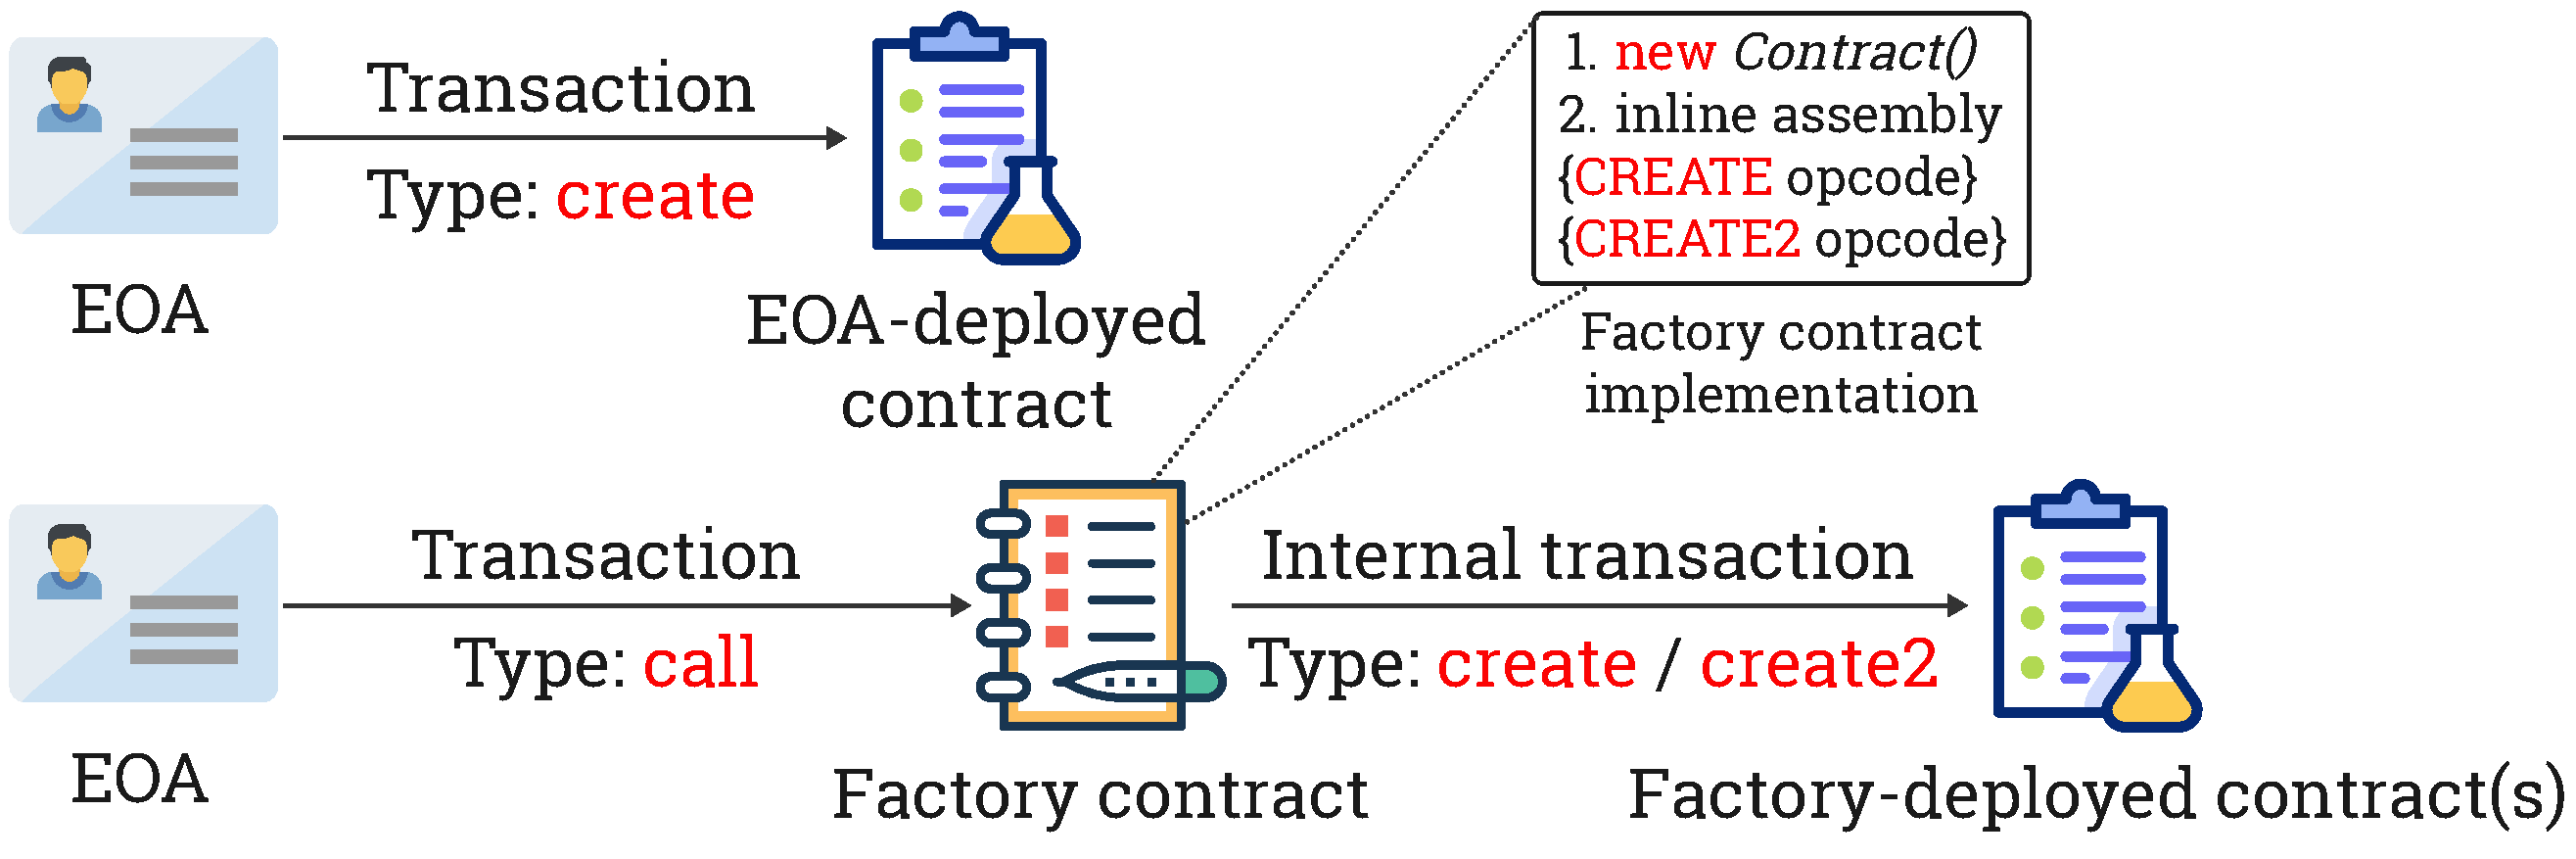
\includegraphics[width=0.75\linewidth]{figures/factoryvseoa.pdf}
		\caption{Comparison of two smart contract deployment methodologies on EVM-compatible chains.
			(i) Direct EOA deployment: Externally Owned Accounts (EOAs) issue create-type transactions
			to deploy contracts directly on-chain. (ii) Factory-mediated deployment: EOAs invoke factory
			contracts through call-type transactions, which then execute internal create/create2 transactions
			to deploy target contracts. Factory contracts utilize two primary implementation approaches:
			high-level \textit{new Contract()} syntax and low-level inline assembly with CREATE/CREATE2
			opcodes.}
		\label{fig:deployment}
	\end{figure}

	Figure~\ref{fig:deployment} illustrates the comparison between contracts deployed by \underline{E}xternally
	\underline{O}wned \underline{A}ccounts (EOA)~\cite{ETHAccount} and those deployed through a factory
	contract. In a direct EOA deployment, an EOA initiates a create transaction, directly deploying
	a new contract to the blockchain. Conversely, factory deployment involves a two-stage process. First,
	an EOA sends a transaction to the factory contract, invoking a specific method designed to handle
	contract deployment. This transaction includes necessary parameters such as constructor
	arguments for the new contract, Ether (ETH) for initialization, and potentially a salt value, depending
	on the deployment method. The factory contract then initiates an internal transaction, using either
	the \textit{create} or \textit{create2} opcode, to execute the actual contract creation and
	deployment.

	The underlying mechanism of smart contract factories relies on two core EVM opcodes: \textit{create}
	and \textit{create2}. The \textit{create} opcode determines the deployment address using the formula
	\textit{addr = keccak256(rlp(sender, nonce))}, where sender represents the address of the account
	(in this case, the factory contract) creating the new contract, and nonce is the number of transactions
	sent by that account. This approach results in deployment addresses that are dependent on the
	factory's transaction history. The \textit{create2} opcode, introduced through EIP-1014~\cite{eip-1014},
	offers a deterministic and more predictable deployment address calculation: \textit{addr =
		keccak256(0xff, sender, salt, keccak256(init\_code))}. Here, sender is the address of the
	factory contract, salt is a user-defined value (allowing for deterministic deployment), and
	\textit{init\_code} is the initialization code of the contract being deployed. Developers can
	trigger contract creation using the high-level \textit{new Contract()} statement within Solidity,
	which typically compiles to the \textit{create} opcode. Alternatively, developers can directly use
	these opcodes within inline assembly blocks for finer-grained control over the deployment process.

	\section{Empirical Study}
	\label{sec:methodology} This section presents our empirical study, including the approach and
	results.

	\subsection{Research Questions}
	Our study aims to address five research questions that systematically investigate factory-related
	smart contracts across two major EVM-compatible chains.

	\begin{itemize}[leftmargin=0.4cm,topsep=0.1cm]
		\item \textbf{RQ1: Detector Effectiveness}. We evaluate the effectiveness of our factory contract
		detection methodology as the foundation for subsequent analyses. \textit{How accurately
		can we identify factory contracts from bytecode? What is the precision and recall of our
		detection approach? How does our detector perform across different contract types?}

		\item \textbf{RQ2: Contract Prevalence}. We quantify the prevalence and deployment trends of
		factory contracts across EVM-compatible chains. \textit{How prevalent are factory
		contracts in real-world deployments? What are the temporal trends in factory contract deployment?
		How do create and create2 opcode usage patterns evolve over time?}

		\item \textbf{RQ3: Application Domains}. We investigate the primary application domains and use
		cases where factory contracts are deployed. \textit{What are the major application
		domains of factory contracts? How are factory contracts distributed across different blockchain
		sectors? What drives the adoption of factory patterns in specific domains?}

		\item \textbf{RQ4: Implementation Analysis}. We explore the technical implementation patterns
		and functionalities of factory contracts. \textit{What unique functionalities do factory
		contracts possess? What are the prevalent design patterns in factory implementations?
		How do different implementation approaches affect contract deployment efficiency?}

		\item \textbf{RQ5: Attack Vector and Security Issue Analysis}. We examine the security risks
		and vulnerabilities associated with factory-related smart contracts. \textit{What are
		the key attack vectors and security issues in factory contracts? How can these attack vectors
		and vulnerabilities be systematically detected? What are the potential impacts and
		mitigation strategies for identified risks?}
	\end{itemize}

	\begin{figure}[t]
		\centering
		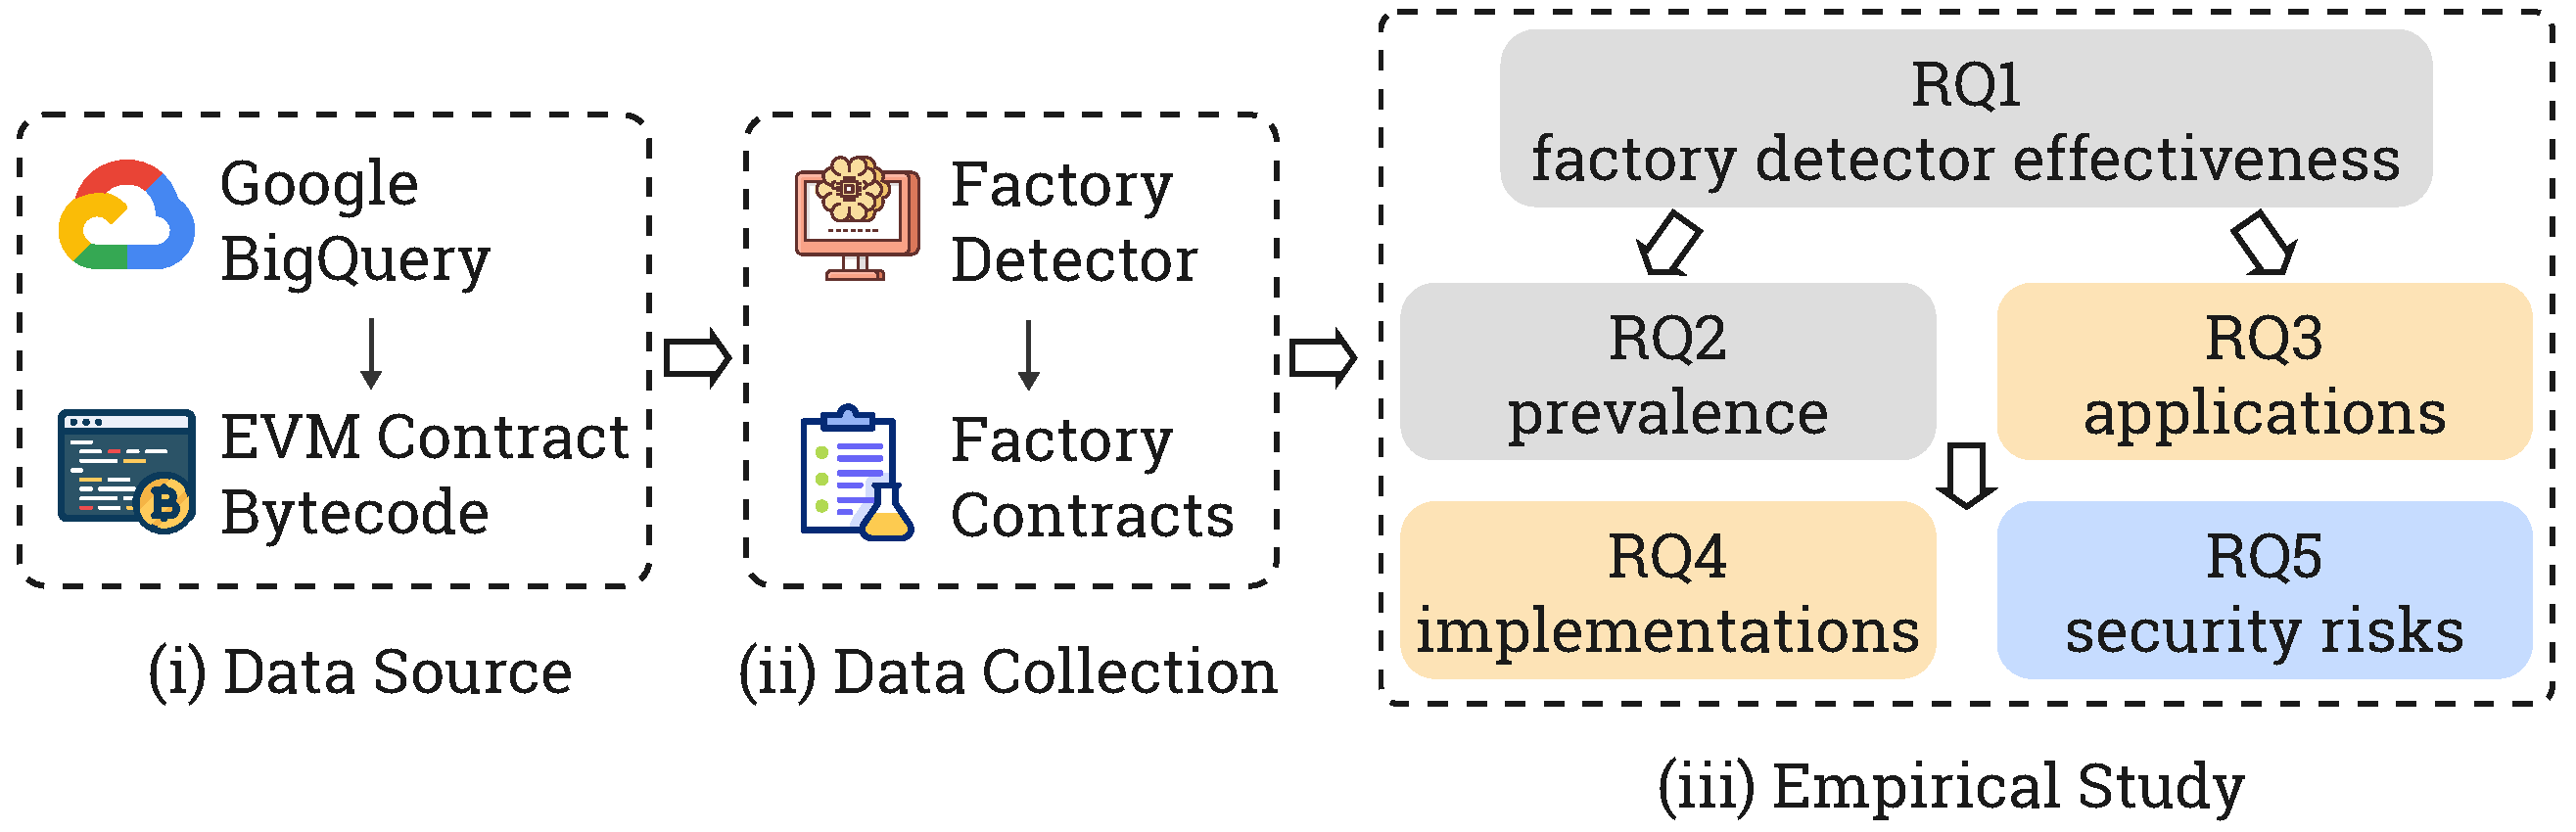
\includegraphics[width=0.85\linewidth]{figures/overview.pdf}
		\caption{Overall workflow of the empirical study across two EVM-compatible chains. (i) Contract
		bytecodes deployed before June 1st, 2025 are extracted from two EVM-compatible chains (Ethereum
		and Polygon) using Google BigQuery. (ii) Factory Contract Detector analyzes all bytecodes to
		identify and collect factory contracts. (iii) The empirical investigation follows five
		sequential research questions, where RQ1 serves as the foundation for subsequent analyses.
		\smash{\colorbox[HTML]{cfcfcf}{\footnotesize Gray blocks}} indicate studies based on contract
		bytecode (RQ1 and RQ2), \smash{\colorbox[HTML]{fde3b6}{\footnotesize orange blocks}} represent
		source code-based analyses (RQ3 and RQ4), and \smash{\colorbox[HTML]{CADCFC}{\footnotesize blue blocks}}
		denote investigations requiring both bytecode and source code (RQ5).}
		\label{fig:workflow}
	\end{figure}

	\subsection{Empirical Study Overview}
	As illustrated in Figure~\ref{fig:workflow}, our empirical study follows a systematic three-phase
	approach to investigate factory-related smart contracts across two EVM-compatible chains.

	\textbf{Phase I: Data Source.} We utilize Google BigQuery~\cite{googlebigquery} as our primary
	data source to extract contract bytecodes from two major EVM-compatible chains: Ethereum~\cite{ethereum}
	and Polygon~\cite{polygon}. We specifically selected these two chains because they are the only
	EVM-compatible chains in Google BigQuery where all contract bytecodes are comprehensively
	available in the BigQuery Public Dataset~\cite{bigquery-public-datasets}. This comprehensive dataset
	provides the foundation for our analysis.

	\textbf{Phase II: Data Collection.} Our Factory Contract Detector analyzes the collected
	bytecodes to systematically identify and extract factory contracts from the multi-chain dataset.
	This automated detection process ensures consistent identification criteria across both blockchain
	chains.

	\textbf{Phase III: Empirical Study.} The investigation follows five sequential research
	questions, where RQ1 (factory detector effectiveness) serves as the methodological foundation for
	subsequent analyses. RQ2-RQ5 examine prevalence, applications, implementations, and security risks
	respectively, utilizing both bytecode-based and source code-based analytical approaches.

	\subsection{Data Source}
	We extract all contract deployed bytecodes\footnote{Deployed bytecode refers to the contract's
	runtime bytecode stored on-chain after deployment, excluding constructor code and initialization
	parameters.} deployed before June 1st, 2025 from Ethereum (mainnet)~\cite{ethereum} and Polygon~\cite{polygon}.
	As shown in Table~\ref{tab:dataset}, our dataset comprises 434,542,165 total contracts with 3,680,947
	unique bytecodes across the two chains, with Ethereum contributing 73,390,233 contracts (1,672,444
	unique bytecodes) and Polygon contributing 361,151,932 contracts (2,008,503 unique bytecodes).

	\newcolumntype{R}{>{\raggedleft\arraybackslash}X} % Define the "R" column type
\begin{table}[t]
	\centering
	\footnotesize
	\caption{Dataset Overview}
	\label{tab:dataset}
	\begin{tabularx}
		{0.6\linewidth}{@{}lRR@{}} \toprule \textbf{Chain} & \textbf{Total Contract} & \textbf{Unique
		Bytecode} \\ \midrule Ethereum & 73,390,233 & 1,672,444 \\ Polygon & 361,151,932 & 2,008,503
		\\ Total & 434,542,165 & 3,680,947 \\ \bottomrule
	\end{tabularx}
\end{table}


	\subsection{Factory Contract Detector}
	Our factory contract detector employs control flow graph (CFG) analysis on deployed bytecode to
	accurately identify factory smart contracts. The detector's core algorithm is presented in Algorithm~\ref{alg:factory_detector}.
	Specifically, the detector constructs a control flow graph from the deployed bytecode by first disassembling
	it into EVM instructions and identifying basic blocks. Each basic block represents a sequence of
	instructions with a single entry and exit point. The algorithm then performs reachability analysis
	from the contract's entry point to determine which basic blocks are executable during contract execution.
	Finally, the detector examines only reachable basic blocks for \textit{CREATE} and \textit{CREATE2}
	operations, ensuring that contract deployment instructions found in data segments or unreachable
	code paths do not result in false positive detections.

	\subsection{Factory Contract Collection}
	Our factory contract collection system systematically gathers factory contracts from two EVM-compatible
	blockchains. Each contract is analyzed using our detector, with results stored including factory
	classifications (Non-factory, CREATE-only, CREATE2-only, or Both) and execution time.

	\subsection{RQ1: Detector Effectiveness}
	This research question aims to evaluate the effectiveness of our Factory Contract Detector through
	metrics including precision, recall, and execution efficiency. Validating the detector's
	effectiveness is crucial as it ensures the accuracy and reliability of our factory contract
	identification, which forms the foundation for all subsequent analyses (RQ2-RQ5).

	\textbf{Ground-Truth Dataset Construction.} We construct a ground-truth dataset to evaluate
	detector effectiveness through two complementary approaches. (i) For factory contracts, we
	utilize Google BigQuery's Ethereum \textit{traces} table~\cite{bigquery-ethereum-traces} to identify
	contracts that executed CREATE or CREATE2 operations in non-constructor contexts with successful
	status, ensuring definitive factory classification through on-chain execution records. (ii) For non-factory
	contracts, we obtain verified smart contracts from Etherscan~\cite{etherscan-verified-contracts}
	and filter those whose source code contains no ``new'', ``create'', or ``create2'' keywords, guaranteeing
	non-factory classification. This methodology yields 548 factory contracts with unique bytecode
	and 2359 non-factory contracts with unique bytecode for evaluation.

	\textbf{False Positive Rate and False Negative Rate.} To evaluate the performance of our factory
	detector, we define the following classification categories:
	\begin{itemize}[leftmargin=0.4cm,topsep=0.1cm]
		\item \textbf{TP (True Positive):} The current contract is a factory contract, and the factory
		detector correctly identifies it as a factory contract.

		\item \textbf{FP (False Positive):} The current contract is not a factory contract, but the factory
		detector incorrectly classifies it as a factory contract.

		\item \textbf{FN (False Negative):} The current contract is a factory contract, but the factory
		detector fails to identify it as such.

		\item \textbf{TN (True Negative):} The current contract is not a factory contract, and the factory
		detector correctly identifies it as a non-factory contract.
	\end{itemize}
	We calculate the False Positive Rate (FPR) and False Negative Rate (FNR) metrics to assess our detector's
	effectiveness. FPR = FP/(FP+TN) measures the proportion of non-factory contracts incorrectly
	classified as factories, while FNR = FN/(FN+TP) measures the proportion of factory contracts missed
	by the detector.

	\begin{algorithm}
	[t!]
		\caption{Factory Contract Detector}
		\label{alg:factory_detector}
		\begin{algorithmic}
		[1] \Statex \textbf{Input:} Contract deployed bytecode $bytecode$ \Statex \textbf{Output:}
		Factory detection result with verification details \Procedure{detectFactoryContract}{$bytecode$}
															   \State $instructions \gets \text{disassemble}(bytecode)$ \If{$instructions = \emptyset$}
																															\State \Return $\text{NotFactory}$ \EndIf

															   \State $basic\_blocks \gets \text{buildBasicBlocks}(instructions)$ \State $cfg \gets \text{addControlFlowEdges}
															   (basic\_blocks, instructions)$ \State $reachable \gets \text{performReachabilityAnalysis}
															   (cfg, entry\_point=0)$

															   \State $verified\_creates \gets \emptyset$ \State $verified\_create2s \gets \emptyset$

															   \ForAll{$block \in reachable$} \State
															   $(creates, create2s) \gets \text{extractCreateOperations}(block)$ \State
															   $verified\_creates \gets verified\_creates \cup creates$ \State
															   $verified\_create2s \gets verified\_create2s \cup create2s$ \EndFor

															   \If{$verified\_creates \neq \emptyset$ \textbf{or} $verified\_create2s \neq \emptyset$}
																   \State \Return $\text{FactoryContract}$ \Else \State \Return $\text{NotFactory}$ \EndIf
		\EndProcedure
		\end{algorithmic}
	\end{algorithm}

	Our evaluation on the complete dataset of 2,907 contracts demonstrates exceptional performance
	with a False Positive Rate of \textbf{0.17\%} and a False Negative Rate of \textbf{8.39\%}. Specifically,
	out of 548 factory contracts, our detector correctly identifies 502 (TP = 502) while missing 46 (FN
	= 46). Among 2,359 non-factory contracts, our detector correctly classifies 2,355 (TN = 2,355) but
	incorrectly flags only 4 as factories (FP = 4). The extremely low False Positive Rate indicates
	that our detector rarely misclassifies non-factory contracts, ensuring high reliability in factory
	identification. The moderate False Negative Rate primarily stems from proxy-based factory
	patterns that exceed the scope of static bytecode analysis. subsequent experimental analyses.

	\textbf{False Negative Analysis.} Our analysis of the 46 false negatives reveals that all
	misclassified cases are attributable to proxy-based factory patterns. These contracts delegate their
	factory functionality to implementation contracts through proxy mechanisms, where the actual
	CREATE/CREATE2 operations occur in the delegated bytecode rather than the proxy contract's own
	bytecode. The execution traces confirm that these contracts successfully performed factory operations,
	but our static bytecode analysis cannot directly obtain the addresses of the latest
	implementation contracts associated with proxies, which exceeds the scope of bytecode-level detection.
	This limitation represents the primary constraint of our detector: the inability to analyze proxy-based
	factory architectures where factory functionality is abstracted through delegation patterns.

	\textbf{False Positive Analysis.} Our analysis of the 4 false positives demonstrates
	exceptionally high precision in factory detection. These misclassifications result from our detector
	erroneously interpreting embedded data sequences within the bytecode as CREATE / CREATE2 opcodes.

	\begin{figure}[htbp]
		\centering
		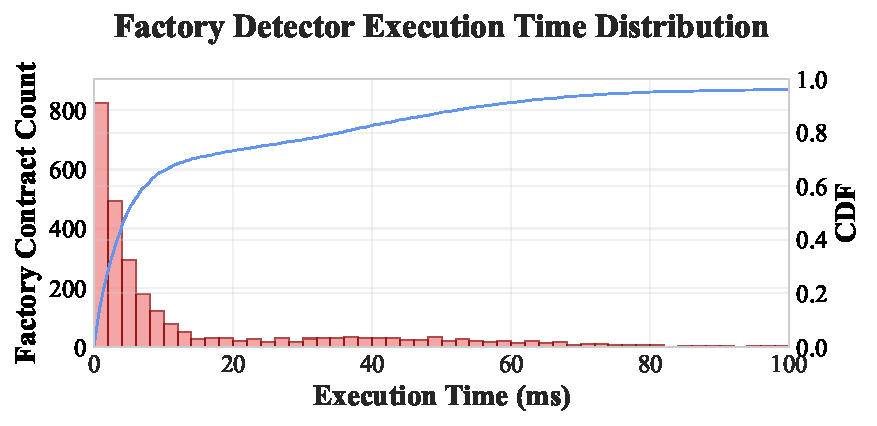
\includegraphics[width=0.7\columnwidth]{figures/execution_time_cdf.pdf}
		\caption{Cumulative Distribution Function (CDF) of execution time for factory contract
		detection across the ground-truth dataset.}
		\label{fig:execution_time_cdf}
	\end{figure}

	\textbf{Execution Performance.} Our factory detector demonstrates excellent computational efficiency
	across the entire ground-truth dataset, as shown in Figure~\ref{fig:execution_time_cdf}. The execution
	time distribution reveals that the majority of contracts are analyzed rapidly, with the
	histogram showing peak frequency in the low-latency range. The cumulative distribution function indicates
	that 25\% of contracts complete analysis within 1.7 milliseconds, while 50\% achieve detection
	in 4.7 milliseconds or less. Furthermore, 75\% of all contracts are processed within 24.2 milliseconds,
	demonstrating the scalability of our approach for large-scale contract analysis.

	\begin{answerbox}
		\textbf{Answer to RQ1:} Our Factory Contract Detector achieves exceptional effectiveness
		with a False Positive Rate of \textbf{0.17\%} and False Negative Rate of \textbf{8.39\%} on
		2,907 contracts. The detector correctly identifies 502/548 factory contracts while misclassifying
		only 4/2,359 non-factory contracts. False negatives stem from proxy-based patterns beyond
		static analysis scope; false positives result from misinterpreting embedded data as CREATE/CREATE2
		opcodes. Performance is excellent with 75\% of contracts analyzed within 24.2 milliseconds.
	\end{answerbox}

	\subsection{RQ2: Prevalence Investigation}

	\begin{figure*}[t]
		\centering
		% (i) Bytecode reuse (top row)
		\begin{minipage}{0.49\textwidth}
			\centering
			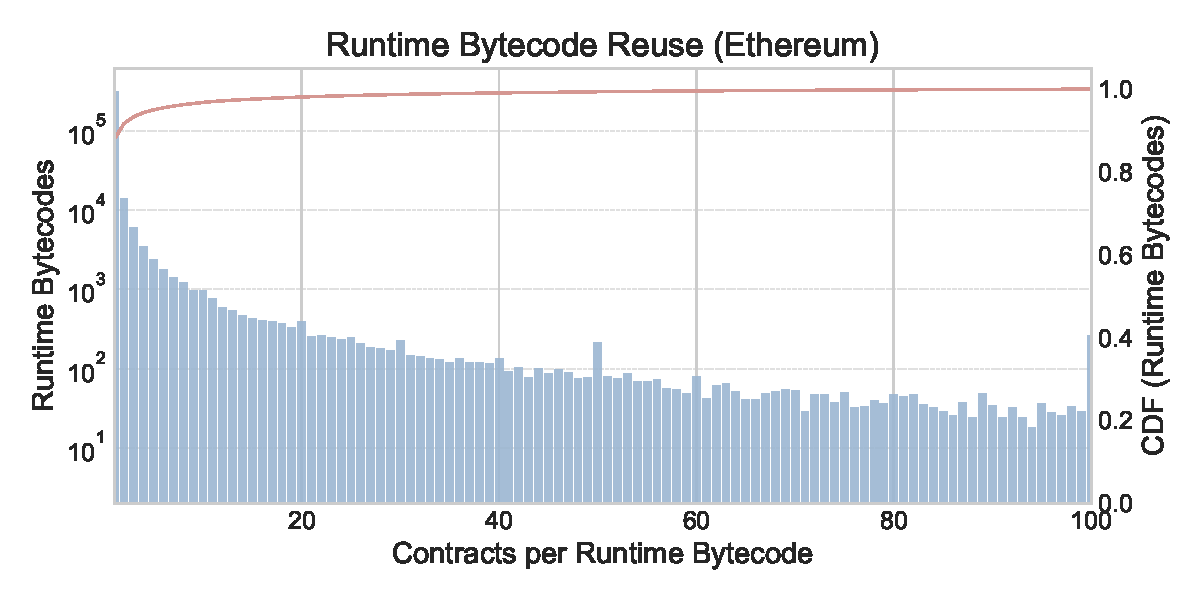
\includegraphics[width=\linewidth]{figures/RQ2/bytecode_reuse_distribution_ethereum.pdf}
		\end{minipage}\hfill
		\begin{minipage}{0.49\textwidth}
			\centering
			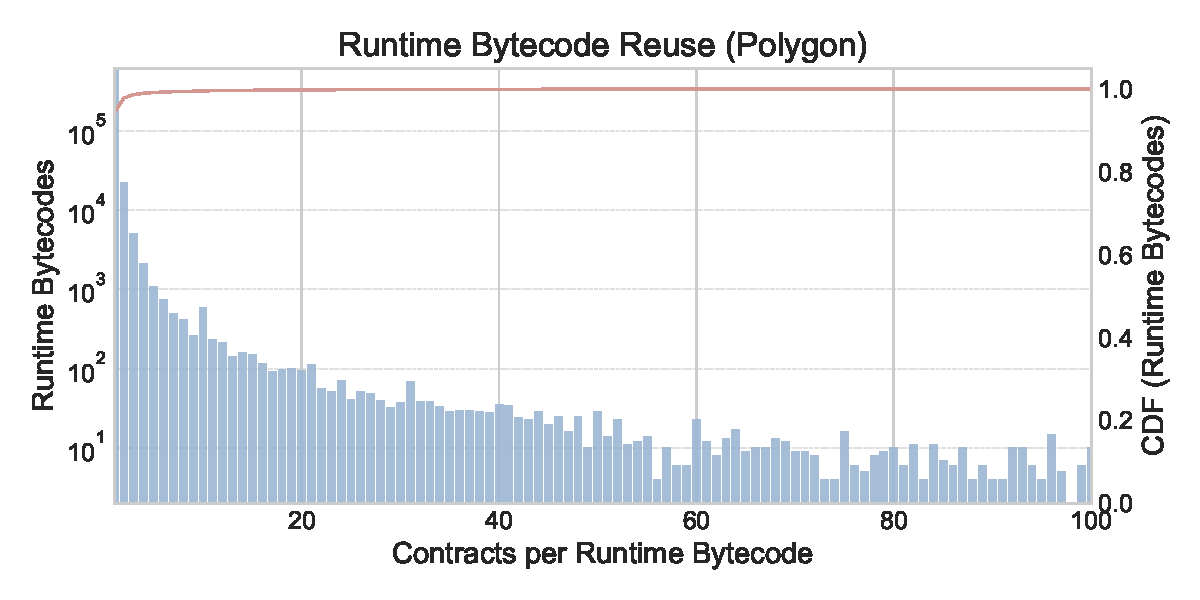
\includegraphics[width=\linewidth]{figures/RQ2/bytecode_reuse_distribution_polygon.pdf}
		\end{minipage}
		\\
		% (ii) Daily active factories (bottom row)
		\begin{minipage}{0.49\textwidth}
			\centering
			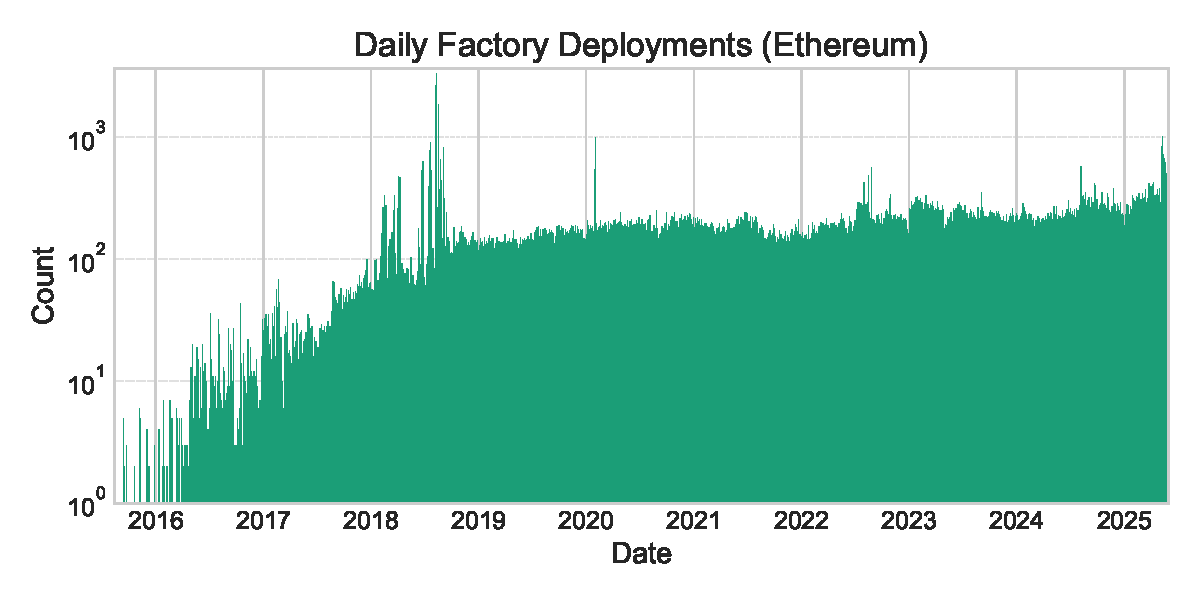
\includegraphics[width=\linewidth]{figures/RQ2/daily_factory_deployments_ethereum.pdf}
		\end{minipage}\hfill
		\begin{minipage}{0.49\textwidth}
			\centering
			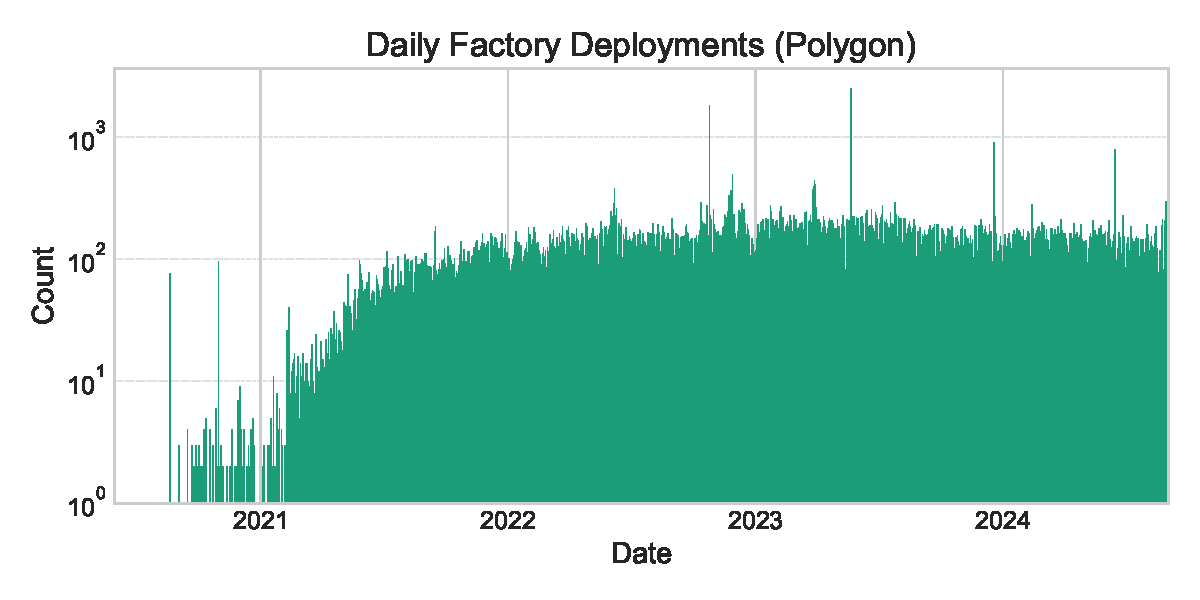
\includegraphics[width=\linewidth]{figures/RQ2/daily_factory_deployments_polygon.pdf}
		\end{minipage}
		\caption{RQ2 (i) and (ii) comparison. Top row: Runtime bytecode reuse distribution (left:
		Ethereum, right: Polygon). X-axis: number of contracts per runtime bytecode (occurrences). Y-axis:
		number of distinct runtime bytecodes with that occurrence count. The overlaid line shows the
		cumulative distribution (CDF). Bottom row: Daily active factories. X-axis: date. Y-axis:
		count of unique factory contracts that executed at least one CREATE/CREATE2 on that day.}
		\label{fig:rq2_group1}
	\end{figure*}

	\textbf{(i) Runtime bytecode reuse.} Both chains show extreme reuse with a long tail (Figure~\ref{fig:rq2_group1},
	top). On Ethereum there are \textbf{362{,}813} distinct runtime bytecodes; \textbf{86.61\%} of them
	(314{,}268/362{,}813) appear only once, covering merely \textbf{0.43\%} of factory-created contracts
	(314{,}268/72{,}881{,}396). In contrast, runtime bytecodes with reuse\,$\ge$\,100 cover \textbf{98.89\%}
	of contracts, and just \textbf{0.30\%} of runtime types (reuse\,$\ge$\,1000) cover \textbf{97.32\%}.
	Polygon is similar: \textbf{626{,}702} runtimes in total; \textbf{94.06\%} appear once yet cover
	only \textbf{5.36\%} of contracts; reuse\,$\ge$\,100 covers \textbf{92.97\%}, and only \textbf{0.04\%}
	of runtime types (225/626{,}702, reuse\,$\ge$\,1000) cover \textbf{91.06\%}. A tiny set of
	templated runtimes dominate the vast majority of factory-created contracts.

	\textbf{(ii) Daily active factories.} As shown in Figure~\ref{fig:rq2_group1} (bottom), both
	chains have stable medians with occasional spikes. Ethereum has activity on \textbf{3{,}476}
	days (2015-08-13 to 2025-05-31), averaging \textbf{152} active factories per day (median \textbf{160},
	95th \textbf{286}); the maximum is \textbf{3{,}342} on 2018-08-10. Polygon spans \textbf{1{,}421}
	days (2020-05-30 to 2024-09-01), averaging \textbf{126} (median \textbf{127}, 95th \textbf{221});
	the maximum is \textbf{2{,}526} on 2023-05-22.

	\textbf{(iii) Daily factory-issued CREATE/CREATE2 deployments.} Figure~\ref{fig:rq2_group2} shows
	that Ethereum factories mint \textbf{20{,}967} contracts per day on average through internal
	CREATE/CREATE2 traces (median \textbf{10{,}662}, 95th \textbf{76{,}617}), peaking at \textbf{267{,}857}
	new contracts on 2020-11-29. Polygon factories average \textbf{8{,}200} deployments per day via
	CREATE/CREATE2 (median \textbf{2{,}674}, 95th \textbf{32{,}506}), with a peak of \textbf{250{,}203} on
	2022-10-26.

	\textbf{(iv) Per-factory cumulative activity.} Figure~\ref{fig:rq2_group2} (bottom) summarizes lifetime
	CREATE/CREATE2 per factory. On Ethereum there are \textbf{120{,}204} factories; \textbf{65.56\%}
	created exactly once, \textbf{90.47\%} created at most 10 times, and \textbf{2.97\%} created \,$\ge$\,100
	times. The mean is \textbf{606} creates/factory, yet creation volume is highly concentrated: the
	top \textbf{50} factories (\textbf{0.04\%}) account for \textbf{80\%} of creates. Polygon has
	\textbf{69{,}258} factories; \textbf{65.07\%} created once, \textbf{91.99\%} at most 10, \textbf{2.50\%}
	\,$\ge$\,100; mean \textbf{168}. The top \textbf{21} factories (\textbf{0.03\%}) cover \textbf{80\%}
	of creates.

	\begin{figure*}[t]
		\centering
		% (iii) Daily create traces (top row)
		\begin{minipage}{0.49\textwidth}
			\centering
			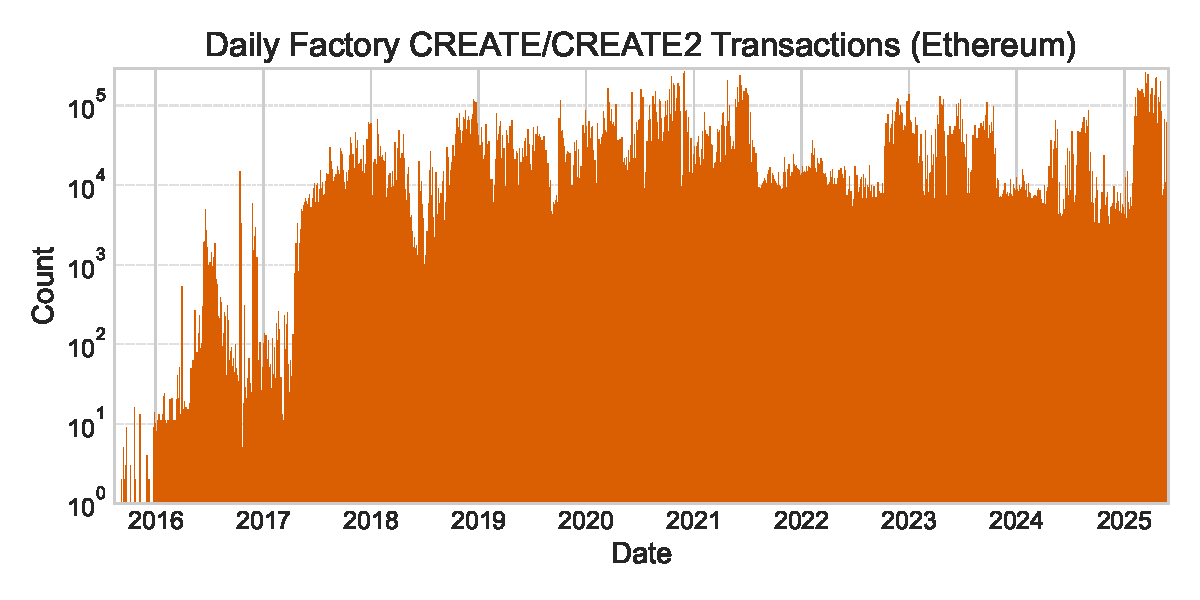
\includegraphics[width=\linewidth]{figures/RQ2/daily_factory_create_traces_ethereum.pdf}
		\end{minipage}\hfill
		\begin{minipage}{0.49\textwidth}
			\centering
			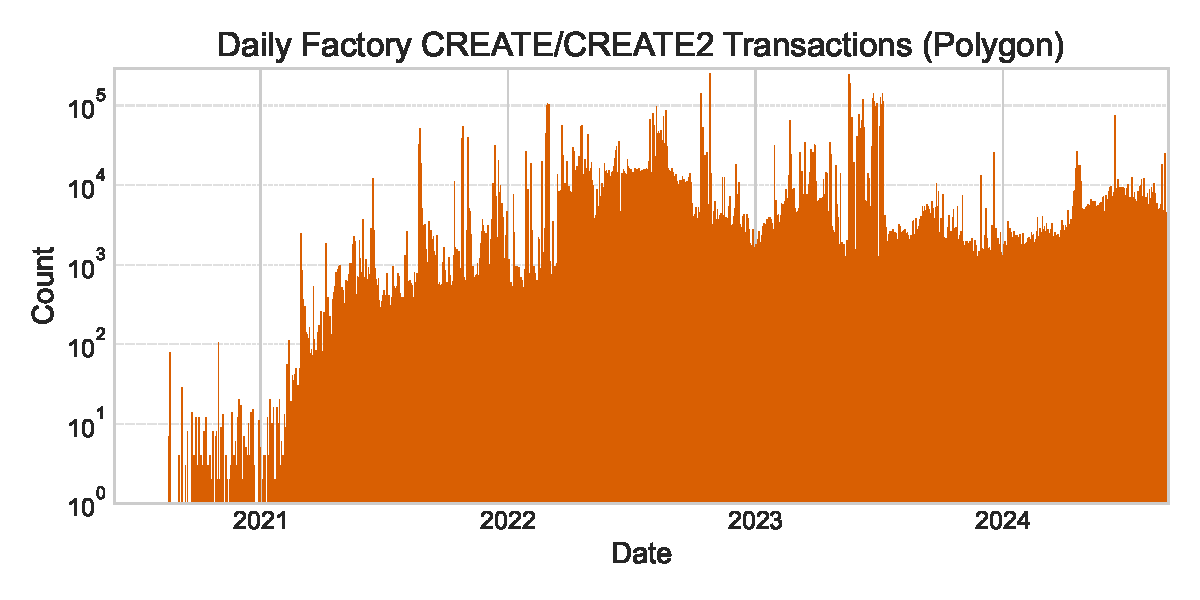
\includegraphics[width=\linewidth]{figures/RQ2/daily_factory_create_traces_polygon.pdf}
		\end{minipage}
		\\
		% (iv) Per-factory total activity (bottom row)
		\begin{minipage}{0.49\textwidth}
			\centering
			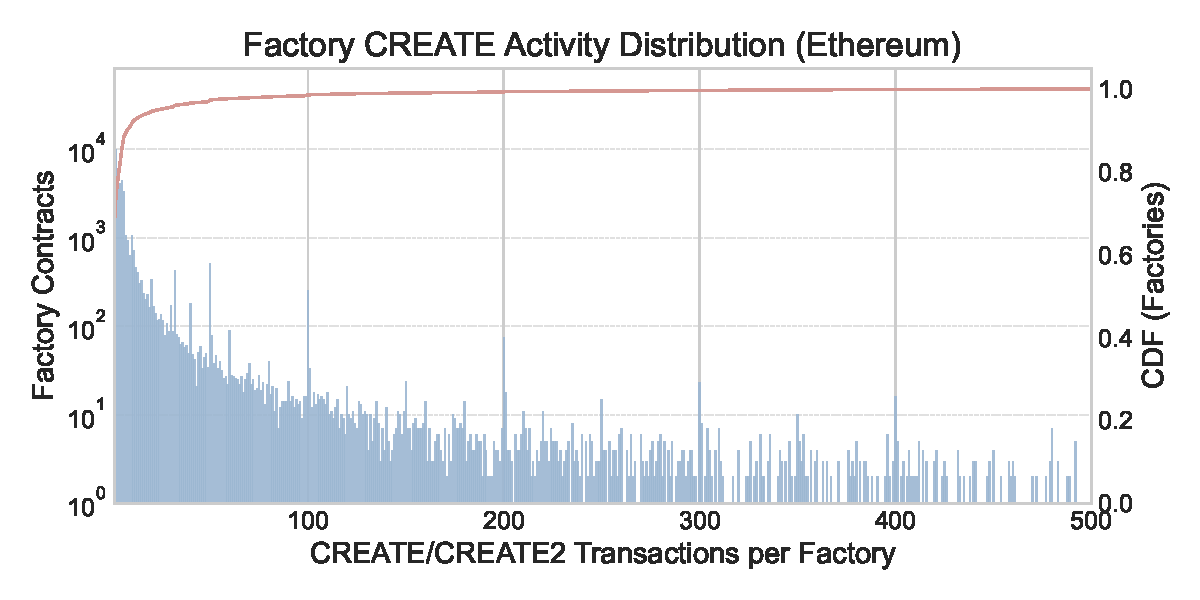
\includegraphics[width=\linewidth]{
				figures/RQ2/factory_activity_distribution_ethereum.pdf
			}
		\end{minipage}\hfill
		\begin{minipage}{0.49\textwidth}
			\centering
			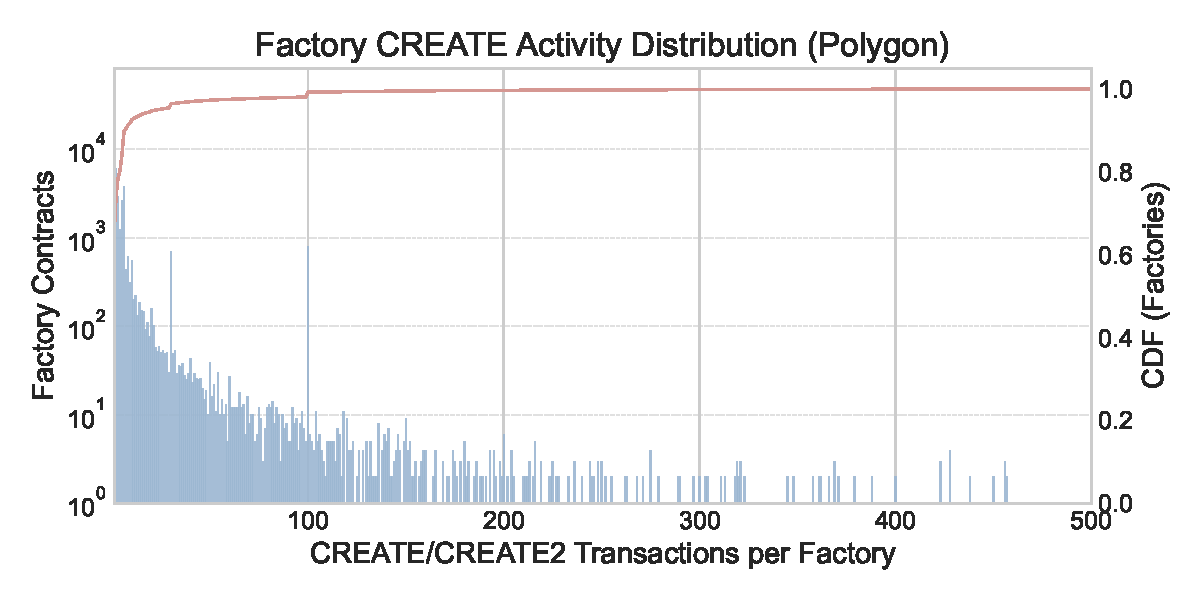
\includegraphics[width=\linewidth]{
				figures/RQ2/factory_activity_distribution_polygon.pdf
			}
		\end{minipage}
		\caption{RQ2 (iii) and (iv) comparison. Top row: Daily factory-issued CREATE/CREATE2 deployments.
		X-axis: date. Y-axis: number of internal CREATE/CREATE2 traces (contracts minted by factories) on
		each day. Bottom row: Per-factory cumulative CREATE/CREATE2 distribution. X-axis: total CREATE/CREATE2
		per factory (lifetime). Y-axis: number of factories. The overlaid line shows the cumulative distribution
			(CDF).}
		\label{fig:rq2_group2}
	\end{figure*}

	\begin{answerbox}
		\textbf{Answer to RQ2:} Factory deployments are highly templated and concentrated. A tiny fraction
		of runtime types (\,$\le$\,\textbf{0.30\%}\,) covers \textbf{91--97\%} of factory-created contracts
		on Ethereum and Polygon, while most runtimes are singletons with negligible coverage. Daily activity
		is steady with substantial throughput (ETH median \textbf{160} factories and \textbf{10{,}662}
		creates/day; POLY \textbf{127} and \textbf{2{,}674}). Creation is extremely skewed: the top
		\textbf{50} (ETH) and \textbf{21} (POLY) factories produce \textbf{80\%} of creates.
	\end{answerbox}

	\subsection{RQ3: Application Domains}
	We sample verified factory contracts from the RQ2 factory table: addresses are sorted by factory
	activity and we take the top \textbf{3,000} with verified source contracts. From each Solidity contract
	we extract multi-view features capturing code semantics and mechanisms, including: (i) name tokens
	from declared contract names; (ii) size/structure signals (lines of code, numbers of contracts/interfaces,
	constructors, modifiers, and imports); (iii) mechanism flags (create/create2/clone/ predict/salt/delegatecall);
	(iv) access-control and library usage (Ownable/AccessControl/onlyOwner, OpenZeppelin and common libraries
	via using-for directives); (v) business keywords (dex, token, nft, wallet, dao, proxy, uups, beacon,
	etc.) and visibility ratios. We standardize features and apply PCA with Varimax rotation, then
	cluster the rotated components using KMeans (k=4). For visualization we embed the data with t-SNE,
	aggregate identical feature vectors, and hide the farthest 10\% points per cluster for clarity. The
	combined map is shown in Figure~\ref{fig:rq3_cluster_map} and the category summary in Table~\ref{tab:clustering-results}.

	\begin{table}[t]
	\centering
	\setlength{\extrarowheight}{1pt}
	\caption{Clustering results for application domains (K=4).}
	\label{tab:clustering-results} \footnotesize
	\begin{tabular}{|m{0.18\textwidth}|m{0.48\textwidth}|>{\centering\arraybackslash}m{0.16\textwidth}|}
		\hline
		\textbf{Category}          & \textbf{Keywords / Signals}                                                     & \textbf{Number}  \\
		\hline
		Finance \& Token           & token, ico, sale, vesting, dividend, fee, vault, stake, yield, distribution     & 1{,}909 (63.6\%) \\
		\hline
		Infrastructure \& Protocol & router, pool, pair, registry, manager, governance, dao, bridge, oracle, module  & 554 (18.5\%)     \\
		\hline
		Proxy \& Upgrade           & proxy, upgradeable, delegatecall, router, beacon, uups, clone, factory, create2 & 461 (15.4\%)     \\
		\hline
		NFT \& Creator             & nft, art, mint, creator, collection, royalty, metadata, game                    & 76 (2.6\%)       \\
		\hline
	\end{tabular}
\end{table}


	\textbf{(i) Finance \& Token.} Token issuance and distribution contracts (ICO/airdrop/vesting),
	fee/dividend distribution, staking/vault management. Beyond plain ERC-20 deployment, factories commonly
	parameterize name/symbol/initial supply, fee switches (e.g., fee-on-transfer), treasury or fee recipients,
	and vesting schedules, and often spin up per-project payment splitters or timelocked vaults.
	Strong signals include token/erc vocabulary, Ownable/AccessControl, and templated create/clone
	deployments, together with distribution helpers (airdrop/vesting) and splitter patterns.

	\textbf{(ii) Infrastructure \& Protocol.} Protocol scaffolding such as routers/pools/registries
	and per-pair or per-pool factories used by AMMs and protocol suites. Deployments emphasize deterministic
	addresses (via \textit{create2}) for discoverability, registry-backed lookup, and reproducible
	per-market instances across chains. Characterized by create2/clone, manager/registry naming
	tokens, and usage of Clones/Create2 libraries; auxiliary modules include fee routers, treasuries,
	and keepers.

	\textbf{(iii) Proxy \& Upgrade.} Factories that deploy proxy or minimal-proxy instances and manage
	upgrades. Typical stacks include EIP-1167 minimal proxies, EIP-1967 storage slots, UUPS/Beacon
	patterns, initializer guards, and upgrade-admin timelocks. Dominated by proxy/upgradeable/beacon/uups/\textit{delegatecall}
	signals and upgrade controllers; init data is passed at creation, with admin/owner roles
	centralized in the factory.

	\begin{figure}[t]
		\centering
		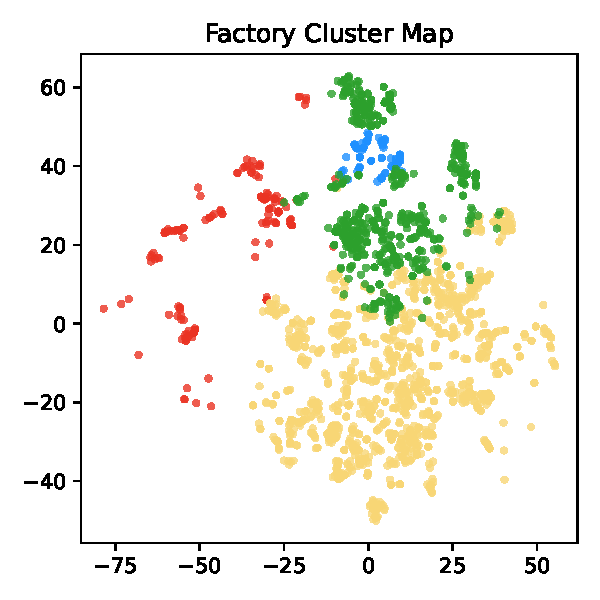
\includegraphics[width=0.45\linewidth]{
			figures/clustered_semantic_space_combined_ethereum_polygon.pdf
		}
		\caption{Factory Cluster Map (K=4) of top-3{,}000 verified factories. Legend: \smash{\colorbox[HTML]{CBEBC6}{\footnotesize green blocks}}
			= Finance \& Token; \smash{\colorbox[HTML]{FDE3B6}{\footnotesize orange blocks}} = Infrastructure
			\& Protocol; \smash{\colorbox[HTML]{CADCFC}{\footnotesize blue blocks}} = Proxy \& Upgrade;
			\smash{\colorbox[HTML]{FAD4D8}{\footnotesize pink blocks}} = NFT \& Creator.}
		\label{fig:rq3_cluster_map}
	\end{figure}

	\textbf{(iv) NFT \& Creator.} Factories for ERC-721/1155-style collections, generative art, and
	games. Common parameters cover baseURI, supply caps, mint price/currency, royalty settings (EIP-2981),
	operator filters, and withdrawal recipients. Signals include mint/collection/royalty/metadata keywords
	with simple access control and drop mechanics (allowlist/Merkle proofs, phased sales, airdrops),
	frequently accompanied by per-collection payment splitters and reveal toggles.

	\begin{answerbox}
		\textbf{Answer to RQ3:} Clustering the top-3,000 verified factory contracts with KMeans (k=4)
		yields four application domains: Finance \& Token (\~63.6\%), Infrastructure \& Protocol (\~18.5\%),
		Proxy \& Upgrade (\~15.4\%), and NFT \& Creator (\~2.6\%). These domains reflect the primary
		intents of factory usage across chains.
	\end{answerbox}
	\subsection{RQ4: Functionalities and Patterns Analysis}

	This study examines factory contract behaviors and implementation patterns. Since analyzing all
	contracts individually is costly, we focus on verified high-volume contracts and involve three smart
	contract security experts for analysis. We follow three systematic steps to uncover factory
	functionalities and implementation patterns: \ding{172} Factory Decomposition - We obtain five
	main smart contract components from Solidity documentation, including State Variables, Functions,
	Modifiers, Events, and Errors, with expert manual review ensuring each functionality correlates
	with multiple contract components. \ding{173} Factory-based Pattern Identification - We explore
	patterns by examining contract semantics, motivations, and functionalities, sourcing Ethereum Improvement
	Proposals related to factory contracts with independent auditing and regular expert meetings.
	\ding{174} Pattern Extraction - We use static analysis to detect patterns in the dataset based on
	syntactic and semantic features. Table~\ref{tab:patterns} details 6 factory-based patterns, their
	motivations, utilized functionalities, and quantities observed in our dataset.

	\textbf{Template Configuration Pattern.} This is the most fundamental pattern in factory
	contracts. It deploys multiple instances of contracts with identical runtime bytecode. The
	pattern dictates that the factory should deploy new contracts based on a predefined template and
	configure new instances via constructor parameters or initialization methods post-deployment. This
	pattern is widely utilized in various dApps, such as ERC-20 token contracts and ERC-721 NFT
	contracts. Two main implementation methods exist: using the \textit{new} keyword (e.g., \textit{new
	Token(strategy, expiration, decimal)}) or using \textit{create} or \textit{create2} in inline
	assembly. For instance, UniswapV2Factory~\cite{uniswapv2factory} shown in Figure~\ref{list:uniswap}
	uses \textit{create2(0,add(),mload(),salt)} to create new pair contracts, followed by
	initialization with \textit{IUniswapV2Pair(p).initialize(t0,t1)}.
	\begin{table}[t]
	\centering
	\setlength{\extrarowheight}{1pt}
	\caption{Identified Factory-based Patterns}
	\label{tab:patterns} \scriptsize
	\begin{tabular}{|m{0.114\textwidth}|m{0.36\textwidth}|m{0.36\textwidth}|}
		\hline
		\textbf{Pattern Name}\centering & \textbf{Motivation}\centering                                                                           & \textbf{Used Functionalities}                                                                                                                                 \\
		\hline
		Template Configuration Pattern  & Facilitate efficient deployment and configuration of identical contracts                                & Use new or \textit{create} / \textit{create2} to deploy contracts. Then call init\_function or pass parameters to the constructor for contract initialization \\
		\hline
		Proxy Delegation Pattern        & Optimize gas costs by deploying minimal proxy contracts for identical contracts                         & Use Clones library to deploy minimized proxy contracts. Validate the untrusted master contract                                                                \\
		\hline
		Centralized Registry Pattern    & Improve management efficiency and traceability of deployed contracts through a centralized approach     & Use \textit{map} / \textit{array} to store and keep track of all deployed contracts. Check which contracts have been previously deployed                      \\
		\hline
		Keyless Singleton Pattern       & Deploy contracts with the same init code to the same address in multiple blockchains                    & Use Nick's method to deploy keyless factories. Utilize \textit{create2} for deterministic contract address independent of deployer's nonce                    \\
		\hline
		Salted Address Pattern          & Calculating the contract address requires only the deployer's address and salt, excluding initcode hash & Utilize \textit{create2} opcode for deterministic contract address independent of deployer account's nonce                                                    \\
		\hline
		Metamorphic Factory Pattern     & Support contract upgradeability and some malicious purposes                                             & Use \textit{selfdestruct} opcode to clear contract code and storage. Use a transient factory to deploy metamorphic contracts                                  \\
		\hline
	\end{tabular}
\end{table}


	\begin{figure}[h]
		\begin{minipage}{0.95\linewidth}
			\begin{lstlisting}
function createPair(address tokenA, address tokenB) external returns (address pair) {
  bytes memory bytecode = type(UniswapV2Pair).creationCode;
  bytes32 salt = keccak256(abi.encodePacked(token0, token1));
  assembly {
    pair := create2(0, add(bytecode, 32), mload(bytecode), salt)
  }
  IUniswapV2Pair(pair).initialize(token0, token1);
  getPair[token0][token1] = pair;
  getPair[token1][token0] = pair;
  allPairs.push(pair);
  emit PairCreated(token0, token1, pair, allPairs.length);
}
			\end{lstlisting}
		\end{minipage}
		\caption{Code snippet of the UniswapV2Factory contract, which uses the bytecode of UniswapV2Pair
		to deploy new trading pair contracts.}
		\label{list:uniswap}
	\end{figure}

	\begin{figure}[h]
		\begin{minipage}{0.95\linewidth}
			\begin{lstlisting}
function cloneDeterministic(address implementation,bytes32 salt,uint256 value) internal{
  assembly ("memory-safe") {
    //Cleans the upper 96 bits of the `implementation` word, then packs the first 3 bytes of the `implementation` add
 ress with the bytecode before the address.
    mstore(0x00, or(shr(0xe8, shl(0x60, implementation)), 0x3d602d80600a3d3981f3363d3d373d3d3d363d73000000))
    //Packs the remaining 17 bytes of `implementation` with the bytecode
    mstore(0x20, or(shl(0x78, implementation), 0x5af43d82803e903d91602b57fd5bf3))
    instance := create2(value, 0x09, 0x37, salt)
  }
  if (instance == address(0)) {
    revert Errors.FailedDeployment();
  }
}
			\end{lstlisting}
		\end{minipage}
		\caption{Code snippet of the OpenZeppelin Clones contract, this function creates a minimal proxy
		of the implementation contract.}
		\label{list:clone}
	\end{figure}

	\textbf{Proxy Delegation Pattern.} \label{sec:proxy-delegation} While the Template Configuration
	Pattern is a simple way to deploy multiple instances, storing the bytecode of each contract repeatedly
	can significantly increase gas costs. This pattern mitigates gas costs associated with storing
	repeated bytecode by deploying one master contract instance. All other instances act as proxies,
	delegating calls to the master while maintaining independent states.

	We analyze the implementation methods and quantities of this pattern in our dataset. Many factories
	use @openzeppelin/contracts/proxy/Clones.sol to deploy minimal proxy contracts. Figure~\ref{list:clone}
	shows the code snippet of the Clones contract, which follows EIP-1167 (Minimal Proxy Contract)~\cite{eip-1167}.
	This factory contract creates a minimal proxy contract of a specified implementation contract, which
	uses minimal bytecode to delegate calls to a fixed address, optimizing gas costs. However,
	unverified master contract addresses could pose security risks, discussed in Section~\ref{sec:security-senderconst}.

	\textbf{Centralized Registry Pattern.} This pattern enhances the management and traceability of
	deployed contracts by using a central registry contract to store the addresses of deployed
	contract instances along with their associated information, such as version and owner details.
	It simplifies the operations of contract factories, making querying and verification more convenient.
	Additionally, it lays the groundwork for advanced functionalities like access control.

	\begin{figure}[h]
		\begin{minipage}{0.95\linewidth}
			\begin{lstlisting}
contract FactoryRegistry {
  mapping(address => address) public proxies;
  mapping(address => bool) public isRegistered;
  address[] public allProxies;
  function registerProxy(address implementation) external returns (address proxy) {
    require(!isRegistered[msg.sender], "Already registered");
    bytes memory bytecode = type(AuthenticatedProxy).creationCode;
    bytes32 salt = keccak256(abi.encodePacked(msg.sender, implementation));
    assembly {
      proxy := create2(0, add(bytecode, 32), mload(bytecode), salt)
    }
    proxies[msg.sender] = proxy;
    isRegistered[msg.sender] = true;
    allProxies.push(proxy);
    AuthenticatedProxy(proxy).initialize(msg.sender, implementation);
  }
}
			\end{lstlisting}
		\end{minipage}
		\caption{Code snippet of a Centralized Registry pattern, managing deployed proxy contracts with
		centralized registration and access control.}
		\label{list:registry}
	\end{figure}

	\textbf{Keyless Singleton Pattern.} Some dapps require deploying contract instances to the deterministic
	address across multiple blockchains, such as contracts adhering to the EIP-1820 (Universal Registry
	Contract)~\cite{eip-1820}. This pattern, proposed in ERC-2470 (Singleton Factory)~\cite{eip-2470},
	and its core involves adopting Nick's method~\cite{nickmethod} to deploy factory contracts. This
	method ensures a deterministic address deployment across blockchains using Nick's method~\cite{nickmethod}.

	Therefore, developers can deploy contract instances with the same initialization code to the same
	address on different chains using such create2 factories. This is because when deploying a
	contract with create2, the contract's address is determined by the factory address, salt, and initcode.
	With the factory address constant across chains, using the same salt ensures the same deployed contract
	address.

	\begin{figure}[h]
		\begin{minipage}{0.95\linewidth}
			\begin{lstlisting}
contract SingletonFactory {
  function deploy(bytes memory _initCode, bytes32 _salt) public returns (address) {
    address addr;
    assembly {
      addr := create2(0, add(_initCode, 0x20), mload(_initCode), _salt)
    }
    require(addr != address(0), "Deploy failed");
    return addr;
  }
  function computeAddress(bytes memory _initCode, bytes32 _salt) public view returns (address) {
    return address(uint160(uint(keccak256(abi.encodePacked(
      byte(0xff),
      address(this),
      _salt,
      keccak256(_initCode)
    )))));
  }
}
			\end{lstlisting}
		\end{minipage}
		\caption{Code snippet of Keyless Singleton pattern, enabling deterministic cross-chain deployment
		using CREATE2 with predictable addresses.}
		\label{list:singleton}
	\end{figure}

	\textbf{Salted Address Pattern.} Some deployers prefer the deployed contract's address not to depend
	on the hash of the initialization code. For this purpose, the EIP-3171~\cite{eip-3171} introduced
	the pattern, called Create3 Factory. This pattern ensures that the address of the deployed contract
	is only determined by the deployer's address and the salt. More importantly, compared to the limitations
	of the Keyless Singleton Pattern, this pattern allows deployers to conveniently deploy contract
	instances with different initialization codes to the same address across multiple blockchains. Additionally,
	contracts deployed through this pattern retain predictability.

	\begin{figure}[h]
		\begin{minipage}{0.95\linewidth}
			\begin{lstlisting}
contract Create3Factory {
  function deploy(bytes32 salt, bytes memory creationCode) external payable returns (address) {
    bytes memory proxyCreationCode = abi.encodePacked(
      hex"67363d3d37363d34f03d5260086018f3",
      creationCode
    );
    address proxy;
    assembly {
      proxy := create2(0, add(proxyCreationCode, 0x20), mload(proxyCreationCode), salt)
    }
    require(proxy != address(0), "Create3: deployment failed");
    return getDeployed(msg.sender, salt);
  }
  function getDeployed(address deployer, bytes32 salt) public pure returns (address) {
    address proxy = address(uint160(uint(keccak256(abi.encodePacked(
      hex"ff", deployer, salt, keccak256(hex"67363d3d37363d34f03d5260086018f3")
    )))));
    return address(uint160(uint(keccak256(abi.encodePacked(hex"d694", proxy, hex"01")))));
  }
}
			\end{lstlisting}
		\end{minipage}
		\caption{Code snippet of Salted Address pattern (Create3), ensuring deployed contract addresses
		depend only on deployer and salt, not initialization code.}
		\label{list:create3}
	\end{figure}

	\textbf{Metamorphic Factory Pattern.} Immutable code is considered to be the cornerstone of a
	stable blockchain ecosystem. However, the emergence of the Metamorphic Factory Pattern disrupts
	this rule. It uses a metamorphic factory to smoothly upgrade factory-deployed contracts without changing
	the deployed contract address, offering viable support for maintenance, fixes, and upgrades
	across multiple chains. Unlike the contract upgrade standards specified by protocols like ERC-1822
	(Universal Upgradeable Proxy Standard)~\cite{eip-1822}, contracts deployed by metamorphic
	factory, once upgraded, will delete all existing storage and replace the existing code with the
	new implementation code. Figure~\ref{lst:metamorphic} presents a concise implementation of metamorphic
	pattern. The \textit{deployMetamorphic()} function utilizes the \textit{create2} opcode to
	deploy TransientFactory. Within the temporary factory's constructor, first deploy the
	metamorphic contract using the create opcode, followed by the execution of a self-destruct operation,
	resetting the transient factory's nonce. When the metamorphic contract needs to be replaced,
	first execute the \textit{selfdestruct} operation on it. Then call the \textit{deployMetamorphic()}
	again, and make sure we pass in the same salt as before. The TransientFactory will redeploy the new
	metamorphic contract code to the same address to achieve the seamless contract replacement.

	\begin{figure}[t]
		\begin{minipage}{0.95\linewidth}
			\begin{lstlisting}
contract MetamorphicContractFactory {
  bytes private transientFactoryCode;
  mapping(address => bytes) private initCodes;
  function deployMetamorphic(bytes32 salt,bytes metamorphicInitCode) external payable {
    address tempFactory;
    assembly {
      let d:=add(0x20, metamorphicInitCode)
      let s:=mload(metamorphicInitCode)
      tempFactory:=create2(callvalue,d,s,salt)
    }
    initCodes[tempFactory]=metamorphicInitCode;
  }
  function getInitCode() external view returns (bytes) {
    return initCodes[msg.sender];
  }
}
contract tempFactory {
  constructor() public payable {
    bytes initCode = IFactory(msg.sender).getInitCode();
    assembly {
      let d := add(0x20,initCode)
      let s := mload(initCode)
      metamorphicAddr := create(callvalue,d,s)
    }
    selfdestruct(metamorphicAddr);
  }
}
			\end{lstlisting}
		\end{minipage}
		\caption{An implementation of metamorphic pattern.}
		\label{lst:metamorphic}
	\end{figure}

	However, this pattern has become a weapon for certain malicious activities, presenting new
	challenges to smart contract security. In Section~\ref{sec:security-mutablecode}, we will
	discuss its attack vectors and corresponding countermeasures in detail.

	\begin{answerbox}
		\textbf{Answer to RQ4:} We systematically identify six distinct factory-based patterns
		through comprehensive analysis of factory contract implementations: Template Configuration Pattern,
		Proxy Delegation Pattern, Centralized Registry Pattern, Keyless Singleton Pattern, Salted Address
		Pattern, and Metamorphic Factory Pattern. These patterns represent fundamental approaches to
		contract deployment, gas optimization, management efficiency, cross-chain deployment, and contract
		upgradeability.
	\end{answerbox}

	\subsection{RQ5: Attack Vector and Security Issue Analysis}
	\label{sec:rq5securityrisks} To assess the security landscape of factory contracts, we conduct a
	systematic analysis to identify and categorize potential Attack Vectors and Security Issues.\footnote{In
	our study, Attack Vector refers to the specific techniques or methods that malicious actors employ
	to exploit factory contract mechanisms for unauthorized purposes, involving manipulation of
	deployment patterns or contract behavior. Security Issue refers to implementation vulnerabilities
	or coding practices in factory contracts that could lead to unintended consequences or compromise
	system security.} Our methodology combines analysis of existing security incident reports and
	Ethereum Improvement Proposals (EIPs) with comprehensive source code examination, involving review
	of documented security incidents, analysis of EIP specifications that introduce new deployment
	mechanisms, and static analysis of factory contract implementations to identify potential vulnerability
	patterns.

	\begin{table}[t]
	\centering
	\footnotesize
	\caption{Classification of Factory Contract Attack Vectors and Security Issues (Type:
	vulnerability classification, Name: specific vulnerability identifier, Code Analysis Level:
	analysis granularity required for identification)}
	\label{tab:attack-vector-security-issue}
	\begin{tabular}{@{}llr@{}}
		\toprule \textbf{Type}                   & \textbf{Name}                             & \textbf{Code Analysis Level} \\
		\midrule \multirow{2}{*}{Attack Vector}  & (1) Mutable Code                          & Bytecode                     \\
		                                         & (2) Address Spoofing Attack               & Bytecode                     \\
		\midrule \multirow{3}{*}{Security Issue} & (1) Unhandled Low-Level Contract Creation & Source Code                  \\
		                                         & (2) Unexpected Ownership Transfer         & Source Code                  \\
		                                         & (3) Unverified Master Contract            & Source Code                  \\
		\bottomrule
	\end{tabular}
\end{table}


	Based on our analysis, we identify two primary attack vectors and three critical security issues
	in factory contract implementations as shown in Table~\ref{tab:attack-vector-security-issue}.
	The following sections provide detailed analysis of each category, including technical analysis,
	real-world case studies, and countermeasures.

	\textbf{Mutable Code:} \label{sec:security-mutablecode} This attack vector exploits the CREATE2
	opcode's deterministic address generation combined with the SELFDESTRUCT operation to achieve
	contract mutability. Attackers deploy a contract at a specific address, destroy it via
	SELFDESTRUCT, then redeploy different code at the same address. This technique enables malicious
	actors to bypass security audits by initially deploying benign contracts that are later replaced
	with malicious versions.

	\textit{Case Study.} The Tornado Cash governance attack exemplifies the Mutable Code vector~\cite{tornado-cash-attack}
	and proceeds as follows (also shown in Figure~\ref{fig:tornado_attack}): \ding{172} \textbf{Benign
	proposal setup via transient factory.} The attacker deploys a transient factory using \textit{CREATE2},
	fixing the factory address by \textit{(deployer, salt, keccak256(init\_code))}. The factory
	deploys a seemingly benign governance proposal at a deterministic address; \ding{173} \textbf{Governance
	approval.} The community/governance process reviews and approves the benign-looking proposal,
	and the address is recorded as the executable proposal; \ding{174} \textbf{Code removal.} The attacker
	triggers \textit{SELFDESTRUCT} on both the transient factory and the benign proposal, deleting their
	code while preserving addresses; \ding{175} \textbf{Factory re-deployment.} Using the same
	\textit{salt} and \textit{init\_code}, the attacker re-deploys the transient factory at the original
	factory address via \textit{CREATE2} (nonce reset); \ding{176} \textbf{Malicious replacement.} The
	re-deployed factory creates a malicious contract at the original proposal address, replacing the
	benign code with attack logic; \ding{177} \textbf{Execution and impact.} When governance executes
	the approved proposal address, it now points to malicious code, enabling fund drainage and unauthorized
	actions.

	\textit{Countermeasures.} Defending against Mutable Code attacks requires a multi-layered
	approach: (i) \textbf{Contract Code Analysis} - Before interacting with any contract, especially
	in governance or high-value transactions, verify that the target contract does not contain
	SELFDESTRUCT opcodes or unreachable SELFDESTRUCT calls through DELEGATECALL operations. This can
	be accomplished through bytecode analysis tools or by requiring contracts to undergo formal verification
	processes that explicitly check for mutability patterns. (ii) \textbf{Deployment Chain
	Validation} - Implement comprehensive validation of the entire contract deployment chain, from
	the target contract back to its ultimate deployer. This involves tracking whether any contract in
	the deployment hierarchy was created using CREATE2, and if so, documenting the salt and bytecode
	parameters used. Governance systems should maintain an immutable record of these parameters to
	detect any attempts at redeployment. (iii) \textbf{Runtime Code Integrity Checks} - Before
	executing any external call or delegating authority to a contract, verify its current extcodehash
	matches the expected value from the initial deployment. This check should be performed
	dynamically, as static analysis alone cannot prevent post-deployment code changes. Smart
	contracts and DApps should implement periodic integrity verification, especially for critical operations
	involving significant value transfers or governance decisions.

	\begin{figure}[t]
		\centering
		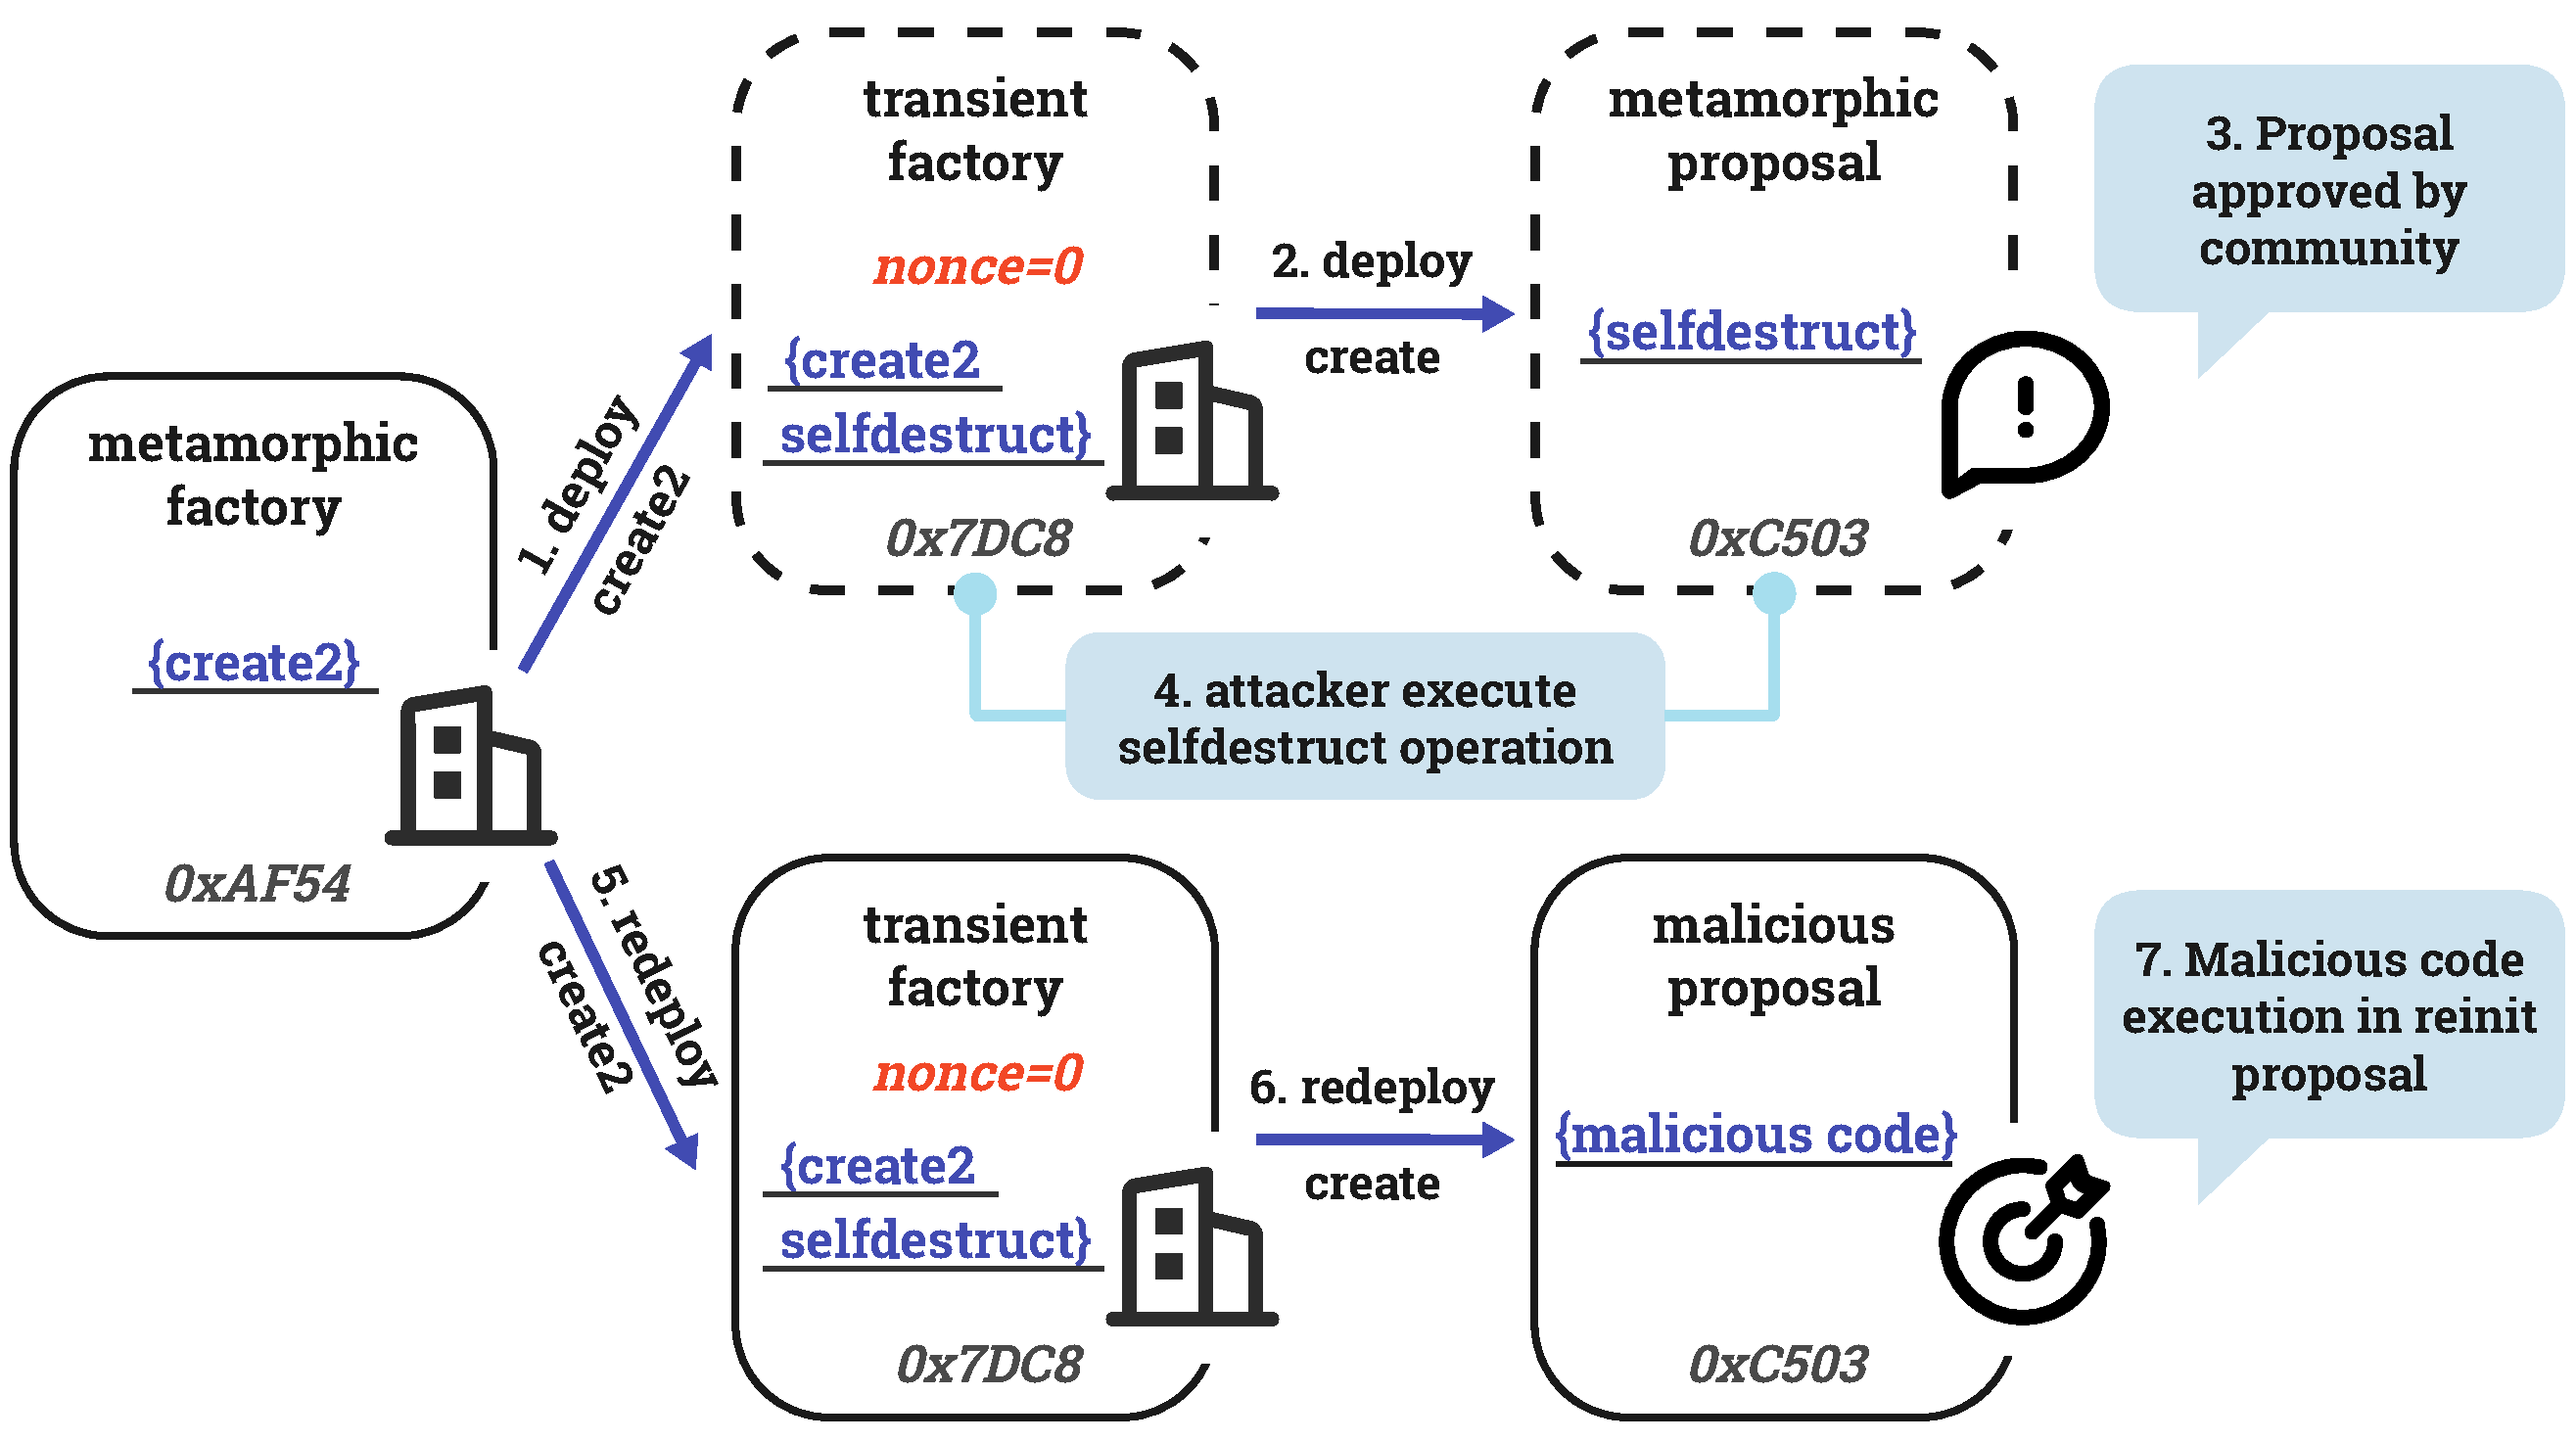
\includegraphics[width=0.85\linewidth]{figures/attack.pdf}
		\caption{The process of Tornado Cash DAO attack.}
		\label{fig:tornado_attack}
	\end{figure}

	\textbf{Address Spoofing Attack:} This attack vector leverages CREATE2's deterministic address computation
	to bypass wallet security alerts that warn users about interactions with known malicious contracts.
	Attackers precompute addresses that appear legitimate or similar to trusted contracts, then deploy
	malicious contracts at these addresses~\cite{scamsniffer-create2-bypass,checkpoint-create2-security}.

	\textit{Case Study.} The Address Spoofing Attack has gained prominence in recent wallet draining
	campaigns, where malicious actors systematically exploit CREATE2's deterministic address generation
	to circumvent security measures~\cite{scamsniffer-create2-bypass,checkpoint-create2-security}.
	In these sophisticated attacks, criminals first identify popular and trusted DeFi protocols,
	then use computational methods to generate thousands of potential addresses that visually
	resemble legitimate contract addresses. For instance, attackers might target a well-known
	decentralized exchange contract whose address begins with "0x1234..." and use CREATE2 with various
	salt values to generate addresses like "0x1234abcd..." or "0x1235defg..." that appear similar at
	first glance. The attack process involves setting up factory contracts specifically designed to
	deploy malicious contracts at these carefully crafted addresses. When users encounter these addresses
	in their wallet interfaces, the visual similarity to trusted contracts can bypass both automated
	security systems that rely on blacklist matching and human verification processes. The malicious
	contracts deployed at these addresses typically contain functions that appear legitimate but include
	hidden backdoors for fund extraction. Some advanced variants of this attack even implement time-based
	triggers, where the malicious functionality only activates after a certain period, making
	initial security audits ineffective.

	\textit{Countermeasures.} Defending against Address Spoofing attacks requires a comprehensive strategy
	that goes beyond simple address comparison: (i) \textbf{Enhanced Address Verification Systems} -
	Wallet providers and DeFi interfaces should implement advanced address verification that examines
	entire addresses rather than just prefixes or suffixes. This includes maintaining comprehensive
	databases of verified contract addresses with their associated metadata, implementing fuzzy matching
	algorithms that can detect visually similar addresses, and providing clear visual indicators
	when users interact with contracts that have addresses similar to known legitimate ones. Additionally,
	implementing address reputation systems that track the deployment history and behavioral
	patterns of contracts can help identify suspicious addresses. (ii) \textbf{User Education and
	Interface Improvements} - Develop educational initiatives to help users understand the risks
	associated with CREATE2-based address manipulation, including providing clear guidelines on how to
	verify contract legitimacy beyond address appearance. Wallet interfaces should display full
	addresses prominently rather than truncating them, implement visual warnings when interacting with
	recently deployed contracts or contracts with similar addresses to known protocols, and provide
	easy access to contract verification status and deployment information. (iii) \textbf{Behavioral
	Analysis and Detection} - Implement real-time monitoring systems that analyze contract
	deployment patterns to identify potential Address Spoofing attempts. This includes tracking the rapid
	deployment of multiple contracts with similar addresses, monitoring for patterns where contracts
	are deployed specifically to mimic existing successful protocols, and implementing machine learning
	algorithms that can detect anomalous address generation patterns that may indicate malicious intent.

	\textbf{Unhandled Low-Level Contract Creation:} This security issue occurs when factories use
	CREATE or CREATE2 opcodes within inline assembly without properly validating the deployment
	result. Unlike high-level deployment using the 'new' keyword which reverts on failure, low-level
	opcodes return zero address on failure while allowing transaction execution to continue. This can
	result in permanent loss of funds if Ether is attached to failed deployments.

	\textit{Case Study.} Unhandled Low-Level Contract Creation represents a critical vulnerability
	that has affected numerous factory contracts in production environments, leading to significant financial
	losses and operational failures. This issue primarily manifests when developers use inline
	assembly with CREATE or CREATE2 opcodes without implementing proper failure handling mechanisms.
	Unlike Solidity's high-level `new` keyword which automatically reverts on deployment failures,
	low-level opcodes return a zero address (0x0) when deployment fails while allowing transaction
	execution to continue. The vulnerability becomes particularly dangerous when combined with value
	transfers, as Ether sent to failed deployments can be permanently lost. A notable real-world example
	occurred in several DeFi factory contracts where developers attempted to optimize gas costs by using
	inline assembly for contract deployment. In one documented case, a factory contract designed to deploy
	lending pool contracts experienced multiple deployment failures due to out-of-gas conditions during
	periods of network congestion. Because the factory code lacked proper validation of the returned
	address from the CREATE2 operation, the contract continued execution and marked the zero address
	as a successfully deployed lending pool in its registry. Subsequent attempts by users to
	interact with these "deployed" contracts resulted in failed transactions, locked funds, and
	significant user experience degradation. The situation was exacerbated by the factory's value transfer
	mechanism, which sent initialization Ether to what it believed were newly deployed contracts but
	were actually null addresses, resulting in irreversible fund losses. Figure~\ref{lst:lowlevel}
	illustrates a more robust approach to this challenge, showing how proper validation can prevent such
	vulnerabilities. The example demonstrates essential safety checks including address validation, pre-deployment
	verification, and post-deployment confirmation that must be implemented when using low-level
	deployment operations.

	\begin{figure}[t]
		\begin{minipage}{0.95\linewidth}
			\begin{lstlisting}
contract Create2Factory {
  mapping(address => bool) deployed;
  function safeCreate2(bytes32 salt,bytes code) external payable {
    address targetAddr = address(uint160(uint256(keccak256(abi.encodePacked(hex"ff",address(this),salt,keccak256(abi.encodePacked(code)))))));
    require(!deployed[targetAddr]);
    assembly {
      let d := add(0x20, code)
      let s := mload(code)
      newAddr := create2(callvalue,d,s,salt)
    }
    require(newAddr == targetAddr);
    deployed[targetAddr] = true;
  }
}
			\end{lstlisting}
		\end{minipage}
		\caption{Example of factory contract using inline assembly with CREATE2 opcode for
		deployment.}
		\label{lst:lowlevel}
	\end{figure}

	\textit{Countermeasures.} Preventing Unhandled Low-Level Contract Creation vulnerabilities
	requires implementing comprehensive validation and error handling mechanisms throughout the
	deployment process: (i) \textbf{Mandatory Return Value Validation} - Always validate that the
	address returned from CREATE or CREATE2 operations is not the zero address (0x0). This can be implemented
	through explicit require statements such as `require(deployedAddress != address(0), "Contract
	deployment failed")` immediately after the assembly block. Additionally, implement address validation
	that checks the returned address matches expected patterns for valid Ethereum addresses,
	ensuring it falls within valid ranges and is not a reserved address. Consider implementing custom
	error types that provide detailed failure information to help with debugging and incident response.
	(ii) \textbf{Deployment Integrity Verification} - After successful address validation, perform
	comprehensive integrity checks to verify the contract was actually deployed correctly. This includes
	verifying that the deployed address contains actual bytecode using `deployedAddress.code.length
	> 0` checks, confirming that the deployed bytecode matches the expected bytecode hash to prevent
	deployment of incorrect contract versions, and implementing pre-computed address validation for CREATE2
	operations by comparing the returned address with the deterministically calculated address. For
	critical applications, consider implementing additional verification through external code hash comparisons
	or checksum validation. (iii) \textbf{State Management and Rollback Mechanisms} - Implement comprehensive
	state management that properly handles deployment failures and prevents inconsistent contract states.
	This includes maintaining deployment status maps that are only updated after successful
	verification of all deployment steps, implementing atomic deployment patterns where all related state
	changes are bundled together and either succeed or fail as a unit, and providing rollback
	mechanisms for partial deployment failures. Additionally, implement event logging for all
	deployment attempts, including failures, to enable proper monitoring and incident response. Consider
	implementing circuit breaker patterns for factory contracts experiencing high deployment failure
	rates to prevent cascade failures and resource exhaustion.

	\begin{figure}[t]
		\begin{minipage}{0.95\linewidth}
			\begin{lstlisting}
abstract contract Ownable is Context {
  address private _owner;
  constructor() {
    transferOwnership(msg.sender);
  }
  function transferOwnership(address newOwner) public onlyOwner {
    require(newOwner != address(0));
    address oldOwner = _owner;
    _owner = newOwner;
  }
}
contract NFTSample is Ownable,ReentrancyGuard {
  constructor() {
    maxBatchSize = 8;
    collectionSize = 16384;
    _setDefaultRoyalty(_owner, 500);
    operatorFilteringEnabled = true;
  }
  function withdrawMoney() onlyOwner {...}
}
			\end{lstlisting}
		\end{minipage}
		\caption{Example of unexpected ownership transfer in factory-deployed contracts.}
		\label{lst:senderinconst}
	\end{figure}

	\textbf{Unexpected Ownership Transfer:} \label{sec:security-senderconst} This security issue arises
	when factory-deployed contracts incorrectly use msg.sender in constructors for ownership assignment.
	Since factories deploy contracts on behalf of users, msg.sender refers to the factory address rather
	than the intended owner, potentially causing loss of access to critical contract functions.

	\textit{Case Study.} The Unexpected Ownership Transfer vulnerability represents one of the most pervasive
	yet subtle security issues affecting factory-deployed contracts, particularly those utilizing
	standard ownership patterns from libraries like OpenZeppelin. This vulnerability has manifested in
	numerous real-world deployments, causing significant operational disruptions and financial
	losses across various DeFi and NFT projects. The core issue arises from a fundamental misunderstanding
	of execution context during contract deployment: when a factory contract deploys a new contract,
	the msg.sender during the constructor execution refers to the factory's address rather than the external
	account that initiated the transaction. This seemingly minor detail has far-reaching
	implications for contracts that rely on msg.sender for access control initialization. A notable example
	occurred in several NFT marketplace factories where thousands of contracts were deployed with incorrect
	ownership assignments. In one documented incident, a popular NFT creation platform deployed over
	10,000 NFT contracts through their factory system, with each contract inheriting from
	OpenZeppelin's Ownable pattern as shown in Figure~\ref{lst:senderinconst}. The contracts were designed
	to allow creators to mint NFTs and withdraw accumulated sales revenue through the withdrawMoney()
	function protected by the onlyOwner modifier. However, due to the Unexpected Ownership Transfer vulnerability,
	the factory contract became the owner of all deployed NFT contracts instead of the intended
	creators. This meant that thousands of NFT creators lost access to critical functions in their contracts,
	including the ability to withdraw funds from sales, modify contract parameters, or execute
	administrative functions. The situation required extensive manual intervention and gas-expensive
	ownership transfer transactions to restore proper access control. In some cases, the factory contract
	itself lacked proper administrative functions to transfer ownership back to the intended users,
	requiring complex upgrade procedures and community coordination to resolve. The vulnerability became
	particularly problematic during high-value NFT drops where significant funds were locked in contracts
	with inaccessible withdrawal functions.

	\textit{Countermeasures.} Preventing Unexpected Ownership Transfer vulnerabilities requires
	implementing robust ownership initialization patterns that account for factory deployment
	contexts: (i) \textbf{Parameter-Based Ownership Initialization} - The most effective approach is
	to modify contract constructors to accept ownership parameters explicitly rather than relying on
	msg.sender. This involves refactoring constructors to include address parameters for the intended
	owner, such as `constructor(address initialOwner)`, and ensuring all inherited contracts (like OpenZeppelin's
	Ownable) are properly initialized with these parameters. Factory contracts should be designed to
	pass tx.origin or explicitly provided owner addresses to deployed contracts during construction.
	This approach provides clear ownership intent and eliminates ambiguity about who should control
	the deployed contract. Additionally, implement validation checks in constructors to ensure that
	provided owner addresses are not zero addresses and represent valid externally owned accounts or
	approved contract addresses. (ii) \textbf{Post-Deployment Ownership Transfer Patterns} - For
	situations where constructor modification is not feasible, implement systematic post-deployment ownership
	transfer mechanisms. This includes designing factory contracts with built-in ownership transfer
	capabilities that automatically call transferOwnership(tx.origin) immediately after successful contract
	deployment, implementing batch ownership transfer functions that can correct ownership for
	multiple contracts simultaneously, and providing emergency recovery mechanisms for cases where initial
	ownership assignment fails. Consider implementing time-locked transfer mechanisms that allow a
	grace period for ownership corrections. Additionally, maintain comprehensive logging of all
	ownership transfer operations to enable audit trails and facilitate troubleshooting.

	\begin{figure}[htbp]
		\begin{minipage}{0.95\linewidth}
			\begin{lstlisting}
import "./proxy/Clones.sol";
contract NinfaFactory is AccessControl {
  using Clones for address;
  mapping(address => bool) collectionWhitelist;
  function cloneCollection(address master,bytes32 salt,bytes data) public {
    require(hasRole(MINTER_ROLE, msg.sender));
    require(collectionWhitelist[master]==true);
    clone = master.cloneDeterministic(salt);
    // bytes4(keccak256('initialize(bytes)'))
    (bool success,) = clone.call(abi.encodeWithSelector(0x439fab91,data));
    require(success);
    emit NewClone(clone, msg.sender);
  }
}
			\end{lstlisting}
		\end{minipage}
		\caption{Example of master contract validation using whitelist and initialization
		verification.}
		\label{lst:checkmaster}
	\end{figure}

	\textbf{Unverified Master Contract:} This security issue affects factories implementing the
	Proxy Delegation Pattern, where externally provided master contract addresses are not properly validated
	before proxy creation. Malicious or incompatible master contracts can compromise the security
	and functionality of all deployed proxies.

	\textit{Case Study.} Figure~\ref{lst:checkmaster} is a simplified version of the NinfaFactory contract
	on the Ethereum mainnet. It serves as a factory for creating NFT distribution contracts. The contract
	imports the Clones library provided by OpenZeppelin to deploy minimal proxies. The
	cloneCollection function takes the master contract's address as a parameter. To ensure the validity
	of the master address, it uses require(collectionWhitelist[master]==true) to check if the master
	contract to be cloned is present in the whitelist. Additionally, the contract uses clone.call(func\_selector)
	to invoke a method of the clone and uses require(success) to verify the result of the function call.

	\textit{Countermeasures.} Defending against unverified master contract vulnerabilities requires
	implementing comprehensive validation mechanisms that ensure both the integrity and
	compatibility of master contracts: (i) \textbf{Whitelist-Based Access Control} - Implement a
	robust whitelist system that maintains a registry of approved master contracts, similar to the NinfaFactory
	example. This system should include role-based access controls (such as ADMIN\_ROLE) for adding
	contracts to the whitelist, regular auditing processes to review and update the whitelist based on
	security assessments, and event logging for all whitelist modifications to maintain transparency.
	The whitelist should store additional metadata about each approved contract, including
	deployment date, audit results, and compatibility version information. (ii) \textbf{Dynamic
	Contract Validation} - Before deploying any proxy, perform comprehensive validation of the master
	contract including verification that the master address contains actual contract code using extcodesize
	checks, validation that the master contract implements expected interfaces through ERC-165 or
	similar standards, and testing critical functions to ensure they exist and behave as expected.
	Implement automated compatibility testing that validates the master contract against known
	function signatures and expected behaviors. (iii) \textbf{Initialization and Post-Deployment
	Verification} - After deploying each proxy, implement comprehensive verification processes to ensure
	proper initialization. This includes validating that the initialization function call succeeds
	and produces expected state changes, implementing comprehensive error handling and revert mechanisms
	if initialization fails, and performing post-deployment verification that the proxy correctly
	delegates to the master contract. Additionally, consider implementing time-locked deployment
	processes where proxies are deployed in a preliminary state and only activated after successful
	verification, providing an opportunity to catch and remediate issues before the contracts become
	operational.

	\begin{answerbox}
		\textbf{Answer to RQ5:} Our analysis identifies two attack vectors (Mutable Code and Address
		Spoofing Attack) that exploit factory contract mechanisms for malicious purposes, and three security
		issues (Unhandled Low-Level Contract Creation, Unexpected Ownership Transfer, and Unverified
		Master Contract) that represent implementation vulnerabilities in factory contracts requiring
		systematic mitigation strategies.
	\end{answerbox}

	\section{Discussions}
	\label{sec:discussions} In this section, we explore some practical implications of our findings,
	discuss potential threats to their validity, and outline directions for future work.

	\subsection{Call to Actions}
	\textit{(i) For Decentralized Governance Committees.} The Tornado Cash incident shows that
	benign-looking proposals can be swapped via metamorphic techniques after approval. Committees should
	reject proposals whose deployment chain contains \textit{selfdestruct}/\textit{delegatecall} or whose
	code provenance cannot be verified end to end (factory address, salt, and init\_code hash should
	all be auditable and consistent). Proposers ought to attest and freeze these deployment
	parameters on-chain prior to voting, and the same values should be verified again at execution.
	A time-locked execution with a short post-approval audit window further reduces risk by allowing
	re-verification that the code at the proposal address still matches the reviewed version.

	\textit{(ii) For Wallet Providers, Security Tools, and dApp Frontends.} Address Spoofing via \textit{CREATE2}
	abuses approvals to undeployed “predicted” addresses. Wallets should flag and require explicit confirmation
	whenever an approval/permit targets a spender with no code (\textit{EXTCODESIZE=0}), and default
	such approvals to bounded amount and duration. Risk context should be surfaced: if the spender is
	a predicted \textit{CREATE2} address from a known factory, show the factory address and, when
	available, the attested init\_code hash; warn or block when provenance is absent. Frontends should
	avoid asking users to approve undeployed spenders, prefer deploy-first then approve-after-code-is-present,
	or bind approvals to code identity by displaying and verifying keccak256(runtime\_code). When using
	factories, pre-commit deployment parameters (factory, salt, init\_code hash), emit attestation events,
	and provide verification links. Both wallets and frontends should offer first-class flows to review
	and revoke high-risk approvals (including undeployed or recently deployed spenders) and integrate
	allowlists/denylists curated by reputable communities.

	\textit{(iii) For Contract Deployers.} Weigh factory overheads versus reuse benefits. Proxy delegation
	(Section~\ref{sec:proxy-delegation}) amortizes code storage but requires whitelist management and
	initialization verification. Account for constructor context as in Section~\ref{sec:security-senderconst}:
	initialize ownership via explicit parameters or perform an immediate post-deploy transfer,
	rather than relying on \textit{msg.sender}.

	\textit{(iv) For Contract Developers.} Harden low-level creation logic by validating returned
	addresses, handling create/create2 failures, and emitting events with salts and code hashes to
	aid traceability. When cloning, verify master contracts via whitelists and live calls (Section~\ref{lst:checkmaster})
	and fail fast on mismatches. Prefer vetted libraries (OpenZeppelin’s \textit{Clones}, \textit{Ownable},
	\textit{ReentrancyGuard}), and document deployment chains to aid audits and community review.

	\subsection{Threats to Validity}

	% The threats to construct validity are associated with two facts. First, our empirical study utilized Slither for
	%	compiling and analyzing contract source code. However, there were a total of 139 factory contracts that failed to
	%	compile, which could impact the validity of the measurement results. We found 79 contracts among these encountered
	%	compilation issues due to unresolved inline assembly. We manually removed some inline assembly code without
	%	affecting  measurement results to ensure successful compilation. Second,
	\textit{Construct Validity.} The research on factory-based patterns (Section~\ref{sec:proxy-delegation})
	and the identification of potential security risks (Section~\ref{sec:rq5securityrisks}) involve manual
	assessments. We mitigate this threat as follows. We establish predefined auditing guidelines for
	reviewers (available in our repository~\cite{fscdata}). These guidelines decompose factory
	functionalities into orthogonal components and finer-grained sub-functionalities. After iterative
	validation, we identify nine sub-functionalities. During a manual re-audit, reviewers examine
	each sub-functionality individually and record concrete implementation methods together with
	related contract components. We then conduct a three-round iterative review to derive patterns and
	security risks, with three trained auditors performing independent reviews and voting in each
	round, and regular discussions with a domain expert. Each round supplements or restructures
	previous results, improving completeness and consistency. The review artifacts are publicly
	available~\cite{fscdata}.

	\textit{Internal Validity.} We use Slither to compile and analyze contract source code. A total
	of 139 factory contracts fail to compile, which could affect measurements. We found that 79 of
	these failures are due to unresolved inline assembly. To enable compilation without biasing results,
	we minimally adjusted or stubbed inline assembly that is unrelated to the measured aspects, ensuring
	the core semantics relevant to our analyses remain intact.
	% the rapid updates of the Solidity and

	\textit{External Validity.} External threats concern the generalizability and representativeness
	of the selected data. We focus on two major EVM-compatible chains (Ethereum and Polygon) because
	comprehensive contract data is publicly available (e.g., via BigQuery), which may limit
	immediate generalizability to other ecosystems. We plan to extend our analysis to additional EVM-compatible
	chains as their datasets mature and become more reproducible. As the ecosystem evolves, new factory-related
	deployment patterns (e.g., CREATE3 factories~\cite{eip-3171}) and security considerations continue
	to emerge; we will complement our taxonomy and analyses accordingly. To minimize bias, we curate
	a wide-ranging and reproducible dataset and release both raw and curated factory-contract
	datasets to facilitate reuse and independent validation.

	\section{Related Work}
	\label{sec:relatedwork}

	\subsection{Empirical Studies of Smart Contracts}
	Some empirical studies have delved into smart contracts. Relevant researches concentrate on
	contract deployment~\cite{DBLP:journals/pacmpl/ChaliasosGL22,DBLP:conf/fc/FrowisB22} and factory-related
	patterns~\cite{DBLP:conf/sigsoft/SunXLLL23,DBLP:conf/fc/SalehiCM22}. Chaliasos et al. ~\cite{DBLP:journals/pacmpl/ChaliasosGL22}
	investigate the prevalence of \textit{create} / \textit{create2} instructions. They categorize
	inline assembly fragments into 10 classes, finding that system operations accounted for 75.06\%
	of total fragments, with \textit{create2} being the most common at 45.09\%. Fröwis et al.~\cite{DBLP:conf/fc/FrowisB22}
	explore the impact and usage of the \textit{create2} instruction, finding that 47\% of contract
	accounts use \textit{create2} for deployment after the Constantinople upgrade. They also provide
	a corresponding detection algorithm and identifying 41 metamorphic code accounts. Sun et al.~\cite{DBLP:conf/sigsoft/SunXLLL23}
	discuss the top-reused factory interface and extract two factory patterns in the token exchange
	and issuance domains. However, these studies only focus on a single aspect of factory contracts,
	covering types, patterns, and application domains, without specific attention to factory-based
	deployments themselves. This limitation leaves room for further exploration. Our empirical study
	comprehensively summarizes multiple dimensions, enhancing the understanding of factory contracts
	in practical development.

	Additionally, there are empirical studies focusing on specific features, patterns, and
	application of smart contracts~\cite{DBLP:conf/uss/BodellMD23,DBLP:journals/corr/abs-2309-02391,DBLP:journals/tse/LiaoSZLHJCCZZ23,DBLP:conf/dsn/FynnBP20,DBLP:conf/issta/FangWYWCCLJ23,DBLP:conf/icse/YinZNWWLLG22,10.1145/3548606.3559341}.
	Liu et al.~\cite{10.1145/3548606.3559341} empirically evaluate the real-world impact of EIP-1559
	on transaction fee dynamics, waiting times, and consensus security. Meisami et al.~\cite{DBLP:conf/uss/BodellMD23}
	pioneer the development of a taxonomy for upgradeable contracts and explore the significance, patterns,
	and security issues. Fang et al.~\cite{DBLP:conf/issta/FangWYWCCLJ23} employ NLP and cluster
	analysis to categorize four usages of custom modifiers. Qian et al.~\cite{DBLP:journals/corr/abs-2309-02391}
	conduct a review of various DeFi attacks and systematically evaluate state-of-the-art smart
	contract security detection tools. Our empirical study systematically discusses various dimensions
	of factory contracts in a progressive manner.

	\subsection{Security Analysis of Smart Contracts}
	Given the relevance of smart contracts to the finance, substantial researches~\cite{DBLP:conf/kbse/XueMLSYP20,DBLP:conf/issta/LiaoZCN22,DBLP:conf/issta/GhalebRP22,DBLP:journals/pacmpl/GrechKJBSS18,
		DBLP:conf/uss/0001L21,DBLP:conf/pldi/BrentGLSS20, DBLP:conf/ccs/DuanZPLLX022}
	are conducted in the field of smart contract security analysis. VetSC~\cite{DBLP:conf/ccs/DuanZPLLX022}
	automates DApp safety vetting through UI-guided semantic extraction, graph generation and model
	checking, revealing security risks like expired tickets and double voting. VRust~\cite{DBLP:conf/ccs/CuiZGT022}
	pioneers a vulnerability detection framework tailored for Solana smart contracts, introducing static
	analysis to validate untrustful input accounts specific to stateless programming model.
	SmartDagger~\cite{DBLP:conf/issta/LiaoZCN22} provides a machine-learning-based semantic recovery
	mechanism, supporting the detection of cross-contract reentrancy vulnerabilities at the bytecode
	level. MadMax~\cite{DBLP:journals/pacmpl/GrechKJBSS18} and eTainter~\cite{DBLP:conf/issta/GhalebRP22}
	tackle gas-related security issues.

However, with the diversification of contract patterns and increased composability, these tools
may struggle to identify vulnerabilities that arise in specific context, leaving this aspect relatively
unexplored. USCHunt~\cite{DBLP:conf/uss/BodellMD23} focuses on security issues with proxy-based
upgradeable patterns, identifying six types of vulnerabilities and discovering 2546 insecure contracts
across blockchains. Building on this direction, an ecosystem-scale empirical study of proxy smart
	contracts further characterizes their prevalence, patterns, and security implications across the
	Ethereum ecosystem~\cite{proxy-empirical-ecosystem}. Additionally, SPCon~\cite{DBLP:conf/issta/LiuL0A22}
	and SoMo ~\cite{DBLP:conf/issta/FangWYWCCLJ23} consider security issues related to function
	modifiers. Several studies dedicate to designing and implementing frameworks for smart contract analysis~
	\cite{DBLP:conf/icse/FeistGG19,DBLP:conf/kbse/FerreiraCDA20,DBLP:conf/sp/SoLPLO20}. To the best of
	our knowledge, these tools have not specifically addressed security issues in the factory
	context. Our work fills this gap by thoroughly examining four security issues related to factory
	contracts, providing case studies and outlining their triggering conditions.

	\subsection{Factory Contracts and Deployment Mechanisms}
	Factory contracts and deployment mechanisms have received increasing attention due to their
	impact on determinism, upgradeability, and ecosystem-scale deployment practices. Empirical and measurement
	studies document how low-level deployment instructions and ecosystem conventions shape development
	patterns and risks. Fröwis and Böhme systematically analyze deployments using \textit{create2} and
	report its role in enabling metamorphic behaviors in the wild~\cite{DBLP:conf/fc/FrowisB22}.
	Chaliasos et al. characterize the prevalence of \textit{create}/\textit{create2} in inline assembly
	and provide taxonomy and tooling implications for safe usage~\cite{DBLP:journals/pacmpl/ChaliasosGL22}.
	Sun et al. mine factory interfaces and distill common factory patterns seen across major domains~\cite{DBLP:conf/sigsoft/SunXLLL23}.
	At the ecosystem scale, USCHunt uncovers systemic issues in proxy-based upgradeability~\cite{DBLP:conf/uss/BodellMD23},
	and subsequent work extends this line with an ecosystem-scale empirical study of proxy contracts
	on Ethereum~\cite{proxy-empirical-ecosystem}. From the perspective of deployment engineering,
	research has explored code generation and deployment pipelines for smart contracts~\cite{DBLP:conf/wcre/TsiounisK22},
	and examined gas modeling and optimization that directly influence deployment choices and factory
	adoption~\cite{DBLP:conf/kbse/Li21a,DBLP:journals/jss/SorboLVVC22,DBLP:journals/tosem/AlbertGHRS22}.
	Our work complements these directions with a comprehensive, data-driven analysis of factory prevalence,
	functionality patterns, and security risks in practice.

	\section{Conclusion}
	\label{sec:conclusion} This paper offers the first ecosystem-scale view of smart-contract factory
	activity across Ethereum and Polygon. We implemented a bytecode-level Factory Contract Detector,
	validated it on a ground-truth benchmark, and applied it to 434{,}542{,}165 deployed runtimes to
	surface 120{,}204 Ethereum factories and 69{,}258 Polygon factories together with their factory-created
	contracts. Building on this detector-driven corpus, we uncover three complementary insights. Longitudinal
	measurements show factories minting over 90\% of contracts since 2020, with creation volume concentrated
	in a small set of high-throughput deployers. Clustering of 3,000 verified factories reveals four
	principal application domains spanning finance, infrastructure, proxy upgradeability, and NFT creation.
	Finally, semantic inspection distills six recurring implementation patterns and highlights factory-centric
	attack vectors and security issues that warrant targeted mitigations. These findings equip
	developers with data-driven guidance on when to employ factory patterns, assist auditors in reasoning
	about factory provenance and governance, and motivate researchers to pursue defenses.

	\begin{acks}
		This work is supported by the National Key Research and Development Program of China
		\newline
		(2022YFF0711404), and the 6th “333 Project” Leading Talent Team Project of Jiangsu Province.
	\end{acks}

	%%
	%% The next two lines define the bibliography style to be used, and
	%% the bibliography file.
	\bibliographystyle{ACM-Reference-Format}
	\bibliography{paper}
\end{document}
\endinput
%%
%% End of file `sample-acmsmall.tex'.
